\documentclass[11pt]{article}

    \usepackage[breakable]{tcolorbox}
    \usepackage{parskip} % Stop auto-indenting (to mimic markdown behaviour)
    
    \usepackage{iftex}
    \ifPDFTeX
    	\usepackage[T1]{fontenc}
    	\usepackage{mathpazo}
    \else
    	\usepackage{fontspec}
    \fi

    % Basic figure setup, for now with no caption control since it's done
    % automatically by Pandoc (which extracts ![](path) syntax from Markdown).
    \usepackage{graphicx}
    % Maintain compatibility with old templates. Remove in nbconvert 6.0
    \let\Oldincludegraphics\includegraphics
    % Ensure that by default, figures have no caption (until we provide a
    % proper Figure object with a Caption API and a way to capture that
    % in the conversion process - todo).
    \usepackage{caption}
    \DeclareCaptionFormat{nocaption}{}
    \captionsetup{format=nocaption,aboveskip=0pt,belowskip=0pt}

    \usepackage{float}
    \floatplacement{figure}{H} % forces figures to be placed at the correct location
    \usepackage{xcolor} % Allow colors to be defined
    \usepackage{enumerate} % Needed for markdown enumerations to work
    \usepackage{geometry} % Used to adjust the document margins
    \usepackage{amsmath} % Equations
    \usepackage{amssymb} % Equations
    \usepackage{textcomp} % defines textquotesingle
    % Hack from http://tex.stackexchange.com/a/47451/13684:
    \AtBeginDocument{%
        \def\PYZsq{\textquotesingle}% Upright quotes in Pygmentized code
    }
    \usepackage{upquote} % Upright quotes for verbatim code
    \usepackage{eurosym} % defines \euro
    \usepackage[mathletters]{ucs} % Extended unicode (utf-8) support
    \usepackage{fancyvrb} % verbatim replacement that allows latex
    \usepackage{grffile} % extends the file name processing of package graphics 
                         % to support a larger range
    \makeatletter % fix for old versions of grffile with XeLaTeX
    \@ifpackagelater{grffile}{2019/11/01}
    {
      % Do nothing on new versions
    }
    {
      \def\Gread@@xetex#1{%
        \IfFileExists{"\Gin@base".bb}%
        {\Gread@eps{\Gin@base.bb}}%
        {\Gread@@xetex@aux#1}%
      }
    }
    \makeatother
    \usepackage[Export]{adjustbox} % Used to constrain images to a maximum size
    \adjustboxset{max size={0.9\linewidth}{0.9\paperheight}}

    % The hyperref package gives us a pdf with properly built
    % internal navigation ('pdf bookmarks' for the table of contents,
    % internal cross-reference links, web links for URLs, etc.)
    \usepackage{hyperref}
    % The default LaTeX title has an obnoxious amount of whitespace. By default,
    % titling removes some of it. It also provides customization options.
    \usepackage{titling}
    \usepackage{longtable} % longtable support required by pandoc >1.10
    \usepackage{booktabs}  % table support for pandoc > 1.12.2
    \usepackage[inline]{enumitem} % IRkernel/repr support (it uses the enumerate* environment)
    \usepackage[normalem]{ulem} % ulem is needed to support strikethroughs (\sout)
                                % normalem makes italics be italics, not underlines
    \usepackage{mathrsfs}
    

    
    % Colors for the hyperref package
    \definecolor{urlcolor}{rgb}{0,.145,.698}
    \definecolor{linkcolor}{rgb}{.71,0.21,0.01}
    \definecolor{citecolor}{rgb}{.12,.54,.11}

    % ANSI colors
    \definecolor{ansi-black}{HTML}{3E424D}
    \definecolor{ansi-black-intense}{HTML}{282C36}
    \definecolor{ansi-red}{HTML}{E75C58}
    \definecolor{ansi-red-intense}{HTML}{B22B31}
    \definecolor{ansi-green}{HTML}{00A250}
    \definecolor{ansi-green-intense}{HTML}{007427}
    \definecolor{ansi-yellow}{HTML}{DDB62B}
    \definecolor{ansi-yellow-intense}{HTML}{B27D12}
    \definecolor{ansi-blue}{HTML}{208FFB}
    \definecolor{ansi-blue-intense}{HTML}{0065CA}
    \definecolor{ansi-magenta}{HTML}{D160C4}
    \definecolor{ansi-magenta-intense}{HTML}{A03196}
    \definecolor{ansi-cyan}{HTML}{60C6C8}
    \definecolor{ansi-cyan-intense}{HTML}{258F8F}
    \definecolor{ansi-white}{HTML}{C5C1B4}
    \definecolor{ansi-white-intense}{HTML}{A1A6B2}
    \definecolor{ansi-default-inverse-fg}{HTML}{FFFFFF}
    \definecolor{ansi-default-inverse-bg}{HTML}{000000}

    % common color for the border for error outputs.
    \definecolor{outerrorbackground}{HTML}{FFDFDF}

    % commands and environments needed by pandoc snippets
    % extracted from the output of `pandoc -s`
    \providecommand{\tightlist}{%
      \setlength{\itemsep}{0pt}\setlength{\parskip}{0pt}}
    \DefineVerbatimEnvironment{Highlighting}{Verbatim}{commandchars=\\\{\}}
    % Add ',fontsize=\small' for more characters per line
    \newenvironment{Shaded}{}{}
    \newcommand{\KeywordTok}[1]{\textcolor[rgb]{0.00,0.44,0.13}{\textbf{{#1}}}}
    \newcommand{\DataTypeTok}[1]{\textcolor[rgb]{0.56,0.13,0.00}{{#1}}}
    \newcommand{\DecValTok}[1]{\textcolor[rgb]{0.25,0.63,0.44}{{#1}}}
    \newcommand{\BaseNTok}[1]{\textcolor[rgb]{0.25,0.63,0.44}{{#1}}}
    \newcommand{\FloatTok}[1]{\textcolor[rgb]{0.25,0.63,0.44}{{#1}}}
    \newcommand{\CharTok}[1]{\textcolor[rgb]{0.25,0.44,0.63}{{#1}}}
    \newcommand{\StringTok}[1]{\textcolor[rgb]{0.25,0.44,0.63}{{#1}}}
    \newcommand{\CommentTok}[1]{\textcolor[rgb]{0.38,0.63,0.69}{\textit{{#1}}}}
    \newcommand{\OtherTok}[1]{\textcolor[rgb]{0.00,0.44,0.13}{{#1}}}
    \newcommand{\AlertTok}[1]{\textcolor[rgb]{1.00,0.00,0.00}{\textbf{{#1}}}}
    \newcommand{\FunctionTok}[1]{\textcolor[rgb]{0.02,0.16,0.49}{{#1}}}
    \newcommand{\RegionMarkerTok}[1]{{#1}}
    \newcommand{\ErrorTok}[1]{\textcolor[rgb]{1.00,0.00,0.00}{\textbf{{#1}}}}
    \newcommand{\NormalTok}[1]{{#1}}
    
    % Additional commands for more recent versions of Pandoc
    \newcommand{\ConstantTok}[1]{\textcolor[rgb]{0.53,0.00,0.00}{{#1}}}
    \newcommand{\SpecialCharTok}[1]{\textcolor[rgb]{0.25,0.44,0.63}{{#1}}}
    \newcommand{\VerbatimStringTok}[1]{\textcolor[rgb]{0.25,0.44,0.63}{{#1}}}
    \newcommand{\SpecialStringTok}[1]{\textcolor[rgb]{0.73,0.40,0.53}{{#1}}}
    \newcommand{\ImportTok}[1]{{#1}}
    \newcommand{\DocumentationTok}[1]{\textcolor[rgb]{0.73,0.13,0.13}{\textit{{#1}}}}
    \newcommand{\AnnotationTok}[1]{\textcolor[rgb]{0.38,0.63,0.69}{\textbf{\textit{{#1}}}}}
    \newcommand{\CommentVarTok}[1]{\textcolor[rgb]{0.38,0.63,0.69}{\textbf{\textit{{#1}}}}}
    \newcommand{\VariableTok}[1]{\textcolor[rgb]{0.10,0.09,0.49}{{#1}}}
    \newcommand{\ControlFlowTok}[1]{\textcolor[rgb]{0.00,0.44,0.13}{\textbf{{#1}}}}
    \newcommand{\OperatorTok}[1]{\textcolor[rgb]{0.40,0.40,0.40}{{#1}}}
    \newcommand{\BuiltInTok}[1]{{#1}}
    \newcommand{\ExtensionTok}[1]{{#1}}
    \newcommand{\PreprocessorTok}[1]{\textcolor[rgb]{0.74,0.48,0.00}{{#1}}}
    \newcommand{\AttributeTok}[1]{\textcolor[rgb]{0.49,0.56,0.16}{{#1}}}
    \newcommand{\InformationTok}[1]{\textcolor[rgb]{0.38,0.63,0.69}{\textbf{\textit{{#1}}}}}
    \newcommand{\WarningTok}[1]{\textcolor[rgb]{0.38,0.63,0.69}{\textbf{\textit{{#1}}}}}
    
    
    % Define a nice break command that doesn't care if a line doesn't already
    % exist.
    \def\br{\hspace*{\fill} \\* }
    % Math Jax compatibility definitions
    \def\gt{>}
    \def\lt{<}
    \let\Oldtex\TeX
    \let\Oldlatex\LaTeX
    \renewcommand{\TeX}{\textrm{\Oldtex}}
    \renewcommand{\LaTeX}{\textrm{\Oldlatex}}
    % Document parameters
    % Document title
    \title{Vectors}
    
    
    
    
    
% Pygments definitions
\makeatletter
\def\PY@reset{\let\PY@it=\relax \let\PY@bf=\relax%
    \let\PY@ul=\relax \let\PY@tc=\relax%
    \let\PY@bc=\relax \let\PY@ff=\relax}
\def\PY@tok#1{\csname PY@tok@#1\endcsname}
\def\PY@toks#1+{\ifx\relax#1\empty\else%
    \PY@tok{#1}\expandafter\PY@toks\fi}
\def\PY@do#1{\PY@bc{\PY@tc{\PY@ul{%
    \PY@it{\PY@bf{\PY@ff{#1}}}}}}}
\def\PY#1#2{\PY@reset\PY@toks#1+\relax+\PY@do{#2}}

\@namedef{PY@tok@w}{\def\PY@tc##1{\textcolor[rgb]{0.73,0.73,0.73}{##1}}}
\@namedef{PY@tok@c}{\let\PY@it=\textit\def\PY@tc##1{\textcolor[rgb]{0.25,0.50,0.50}{##1}}}
\@namedef{PY@tok@cp}{\def\PY@tc##1{\textcolor[rgb]{0.74,0.48,0.00}{##1}}}
\@namedef{PY@tok@k}{\let\PY@bf=\textbf\def\PY@tc##1{\textcolor[rgb]{0.00,0.50,0.00}{##1}}}
\@namedef{PY@tok@kp}{\def\PY@tc##1{\textcolor[rgb]{0.00,0.50,0.00}{##1}}}
\@namedef{PY@tok@kt}{\def\PY@tc##1{\textcolor[rgb]{0.69,0.00,0.25}{##1}}}
\@namedef{PY@tok@o}{\def\PY@tc##1{\textcolor[rgb]{0.40,0.40,0.40}{##1}}}
\@namedef{PY@tok@ow}{\let\PY@bf=\textbf\def\PY@tc##1{\textcolor[rgb]{0.67,0.13,1.00}{##1}}}
\@namedef{PY@tok@nb}{\def\PY@tc##1{\textcolor[rgb]{0.00,0.50,0.00}{##1}}}
\@namedef{PY@tok@nf}{\def\PY@tc##1{\textcolor[rgb]{0.00,0.00,1.00}{##1}}}
\@namedef{PY@tok@nc}{\let\PY@bf=\textbf\def\PY@tc##1{\textcolor[rgb]{0.00,0.00,1.00}{##1}}}
\@namedef{PY@tok@nn}{\let\PY@bf=\textbf\def\PY@tc##1{\textcolor[rgb]{0.00,0.00,1.00}{##1}}}
\@namedef{PY@tok@ne}{\let\PY@bf=\textbf\def\PY@tc##1{\textcolor[rgb]{0.82,0.25,0.23}{##1}}}
\@namedef{PY@tok@nv}{\def\PY@tc##1{\textcolor[rgb]{0.10,0.09,0.49}{##1}}}
\@namedef{PY@tok@no}{\def\PY@tc##1{\textcolor[rgb]{0.53,0.00,0.00}{##1}}}
\@namedef{PY@tok@nl}{\def\PY@tc##1{\textcolor[rgb]{0.63,0.63,0.00}{##1}}}
\@namedef{PY@tok@ni}{\let\PY@bf=\textbf\def\PY@tc##1{\textcolor[rgb]{0.60,0.60,0.60}{##1}}}
\@namedef{PY@tok@na}{\def\PY@tc##1{\textcolor[rgb]{0.49,0.56,0.16}{##1}}}
\@namedef{PY@tok@nt}{\let\PY@bf=\textbf\def\PY@tc##1{\textcolor[rgb]{0.00,0.50,0.00}{##1}}}
\@namedef{PY@tok@nd}{\def\PY@tc##1{\textcolor[rgb]{0.67,0.13,1.00}{##1}}}
\@namedef{PY@tok@s}{\def\PY@tc##1{\textcolor[rgb]{0.73,0.13,0.13}{##1}}}
\@namedef{PY@tok@sd}{\let\PY@it=\textit\def\PY@tc##1{\textcolor[rgb]{0.73,0.13,0.13}{##1}}}
\@namedef{PY@tok@si}{\let\PY@bf=\textbf\def\PY@tc##1{\textcolor[rgb]{0.73,0.40,0.53}{##1}}}
\@namedef{PY@tok@se}{\let\PY@bf=\textbf\def\PY@tc##1{\textcolor[rgb]{0.73,0.40,0.13}{##1}}}
\@namedef{PY@tok@sr}{\def\PY@tc##1{\textcolor[rgb]{0.73,0.40,0.53}{##1}}}
\@namedef{PY@tok@ss}{\def\PY@tc##1{\textcolor[rgb]{0.10,0.09,0.49}{##1}}}
\@namedef{PY@tok@sx}{\def\PY@tc##1{\textcolor[rgb]{0.00,0.50,0.00}{##1}}}
\@namedef{PY@tok@m}{\def\PY@tc##1{\textcolor[rgb]{0.40,0.40,0.40}{##1}}}
\@namedef{PY@tok@gh}{\let\PY@bf=\textbf\def\PY@tc##1{\textcolor[rgb]{0.00,0.00,0.50}{##1}}}
\@namedef{PY@tok@gu}{\let\PY@bf=\textbf\def\PY@tc##1{\textcolor[rgb]{0.50,0.00,0.50}{##1}}}
\@namedef{PY@tok@gd}{\def\PY@tc##1{\textcolor[rgb]{0.63,0.00,0.00}{##1}}}
\@namedef{PY@tok@gi}{\def\PY@tc##1{\textcolor[rgb]{0.00,0.63,0.00}{##1}}}
\@namedef{PY@tok@gr}{\def\PY@tc##1{\textcolor[rgb]{1.00,0.00,0.00}{##1}}}
\@namedef{PY@tok@ge}{\let\PY@it=\textit}
\@namedef{PY@tok@gs}{\let\PY@bf=\textbf}
\@namedef{PY@tok@gp}{\let\PY@bf=\textbf\def\PY@tc##1{\textcolor[rgb]{0.00,0.00,0.50}{##1}}}
\@namedef{PY@tok@go}{\def\PY@tc##1{\textcolor[rgb]{0.53,0.53,0.53}{##1}}}
\@namedef{PY@tok@gt}{\def\PY@tc##1{\textcolor[rgb]{0.00,0.27,0.87}{##1}}}
\@namedef{PY@tok@err}{\def\PY@bc##1{{\setlength{\fboxsep}{\string -\fboxrule}\fcolorbox[rgb]{1.00,0.00,0.00}{1,1,1}{\strut ##1}}}}
\@namedef{PY@tok@kc}{\let\PY@bf=\textbf\def\PY@tc##1{\textcolor[rgb]{0.00,0.50,0.00}{##1}}}
\@namedef{PY@tok@kd}{\let\PY@bf=\textbf\def\PY@tc##1{\textcolor[rgb]{0.00,0.50,0.00}{##1}}}
\@namedef{PY@tok@kn}{\let\PY@bf=\textbf\def\PY@tc##1{\textcolor[rgb]{0.00,0.50,0.00}{##1}}}
\@namedef{PY@tok@kr}{\let\PY@bf=\textbf\def\PY@tc##1{\textcolor[rgb]{0.00,0.50,0.00}{##1}}}
\@namedef{PY@tok@bp}{\def\PY@tc##1{\textcolor[rgb]{0.00,0.50,0.00}{##1}}}
\@namedef{PY@tok@fm}{\def\PY@tc##1{\textcolor[rgb]{0.00,0.00,1.00}{##1}}}
\@namedef{PY@tok@vc}{\def\PY@tc##1{\textcolor[rgb]{0.10,0.09,0.49}{##1}}}
\@namedef{PY@tok@vg}{\def\PY@tc##1{\textcolor[rgb]{0.10,0.09,0.49}{##1}}}
\@namedef{PY@tok@vi}{\def\PY@tc##1{\textcolor[rgb]{0.10,0.09,0.49}{##1}}}
\@namedef{PY@tok@vm}{\def\PY@tc##1{\textcolor[rgb]{0.10,0.09,0.49}{##1}}}
\@namedef{PY@tok@sa}{\def\PY@tc##1{\textcolor[rgb]{0.73,0.13,0.13}{##1}}}
\@namedef{PY@tok@sb}{\def\PY@tc##1{\textcolor[rgb]{0.73,0.13,0.13}{##1}}}
\@namedef{PY@tok@sc}{\def\PY@tc##1{\textcolor[rgb]{0.73,0.13,0.13}{##1}}}
\@namedef{PY@tok@dl}{\def\PY@tc##1{\textcolor[rgb]{0.73,0.13,0.13}{##1}}}
\@namedef{PY@tok@s2}{\def\PY@tc##1{\textcolor[rgb]{0.73,0.13,0.13}{##1}}}
\@namedef{PY@tok@sh}{\def\PY@tc##1{\textcolor[rgb]{0.73,0.13,0.13}{##1}}}
\@namedef{PY@tok@s1}{\def\PY@tc##1{\textcolor[rgb]{0.73,0.13,0.13}{##1}}}
\@namedef{PY@tok@mb}{\def\PY@tc##1{\textcolor[rgb]{0.40,0.40,0.40}{##1}}}
\@namedef{PY@tok@mf}{\def\PY@tc##1{\textcolor[rgb]{0.40,0.40,0.40}{##1}}}
\@namedef{PY@tok@mh}{\def\PY@tc##1{\textcolor[rgb]{0.40,0.40,0.40}{##1}}}
\@namedef{PY@tok@mi}{\def\PY@tc##1{\textcolor[rgb]{0.40,0.40,0.40}{##1}}}
\@namedef{PY@tok@il}{\def\PY@tc##1{\textcolor[rgb]{0.40,0.40,0.40}{##1}}}
\@namedef{PY@tok@mo}{\def\PY@tc##1{\textcolor[rgb]{0.40,0.40,0.40}{##1}}}
\@namedef{PY@tok@ch}{\let\PY@it=\textit\def\PY@tc##1{\textcolor[rgb]{0.25,0.50,0.50}{##1}}}
\@namedef{PY@tok@cm}{\let\PY@it=\textit\def\PY@tc##1{\textcolor[rgb]{0.25,0.50,0.50}{##1}}}
\@namedef{PY@tok@cpf}{\let\PY@it=\textit\def\PY@tc##1{\textcolor[rgb]{0.25,0.50,0.50}{##1}}}
\@namedef{PY@tok@c1}{\let\PY@it=\textit\def\PY@tc##1{\textcolor[rgb]{0.25,0.50,0.50}{##1}}}
\@namedef{PY@tok@cs}{\let\PY@it=\textit\def\PY@tc##1{\textcolor[rgb]{0.25,0.50,0.50}{##1}}}

\def\PYZbs{\char`\\}
\def\PYZus{\char`\_}
\def\PYZob{\char`\{}
\def\PYZcb{\char`\}}
\def\PYZca{\char`\^}
\def\PYZam{\char`\&}
\def\PYZlt{\char`\<}
\def\PYZgt{\char`\>}
\def\PYZsh{\char`\#}
\def\PYZpc{\char`\%}
\def\PYZdl{\char`\$}
\def\PYZhy{\char`\-}
\def\PYZsq{\char`\'}
\def\PYZdq{\char`\"}
\def\PYZti{\char`\~}
% for compatibility with earlier versions
\def\PYZat{@}
\def\PYZlb{[}
\def\PYZrb{]}
\makeatother


    % For linebreaks inside Verbatim environment from package fancyvrb. 
    \makeatletter
        \newbox\Wrappedcontinuationbox 
        \newbox\Wrappedvisiblespacebox 
        \newcommand*\Wrappedvisiblespace {\textcolor{red}{\textvisiblespace}} 
        \newcommand*\Wrappedcontinuationsymbol {\textcolor{red}{\llap{\tiny$\m@th\hookrightarrow$}}} 
        \newcommand*\Wrappedcontinuationindent {3ex } 
        \newcommand*\Wrappedafterbreak {\kern\Wrappedcontinuationindent\copy\Wrappedcontinuationbox} 
        % Take advantage of the already applied Pygments mark-up to insert 
        % potential linebreaks for TeX processing. 
        %        {, <, #, %, $, ' and ": go to next line. 
        %        _, }, ^, &, >, - and ~: stay at end of broken line. 
        % Use of \textquotesingle for straight quote. 
        \newcommand*\Wrappedbreaksatspecials {% 
            \def\PYGZus{\discretionary{\char`\_}{\Wrappedafterbreak}{\char`\_}}% 
            \def\PYGZob{\discretionary{}{\Wrappedafterbreak\char`\{}{\char`\{}}% 
            \def\PYGZcb{\discretionary{\char`\}}{\Wrappedafterbreak}{\char`\}}}% 
            \def\PYGZca{\discretionary{\char`\^}{\Wrappedafterbreak}{\char`\^}}% 
            \def\PYGZam{\discretionary{\char`\&}{\Wrappedafterbreak}{\char`\&}}% 
            \def\PYGZlt{\discretionary{}{\Wrappedafterbreak\char`\<}{\char`\<}}% 
            \def\PYGZgt{\discretionary{\char`\>}{\Wrappedafterbreak}{\char`\>}}% 
            \def\PYGZsh{\discretionary{}{\Wrappedafterbreak\char`\#}{\char`\#}}% 
            \def\PYGZpc{\discretionary{}{\Wrappedafterbreak\char`\%}{\char`\%}}% 
            \def\PYGZdl{\discretionary{}{\Wrappedafterbreak\char`\$}{\char`\$}}% 
            \def\PYGZhy{\discretionary{\char`\-}{\Wrappedafterbreak}{\char`\-}}% 
            \def\PYGZsq{\discretionary{}{\Wrappedafterbreak\textquotesingle}{\textquotesingle}}% 
            \def\PYGZdq{\discretionary{}{\Wrappedafterbreak\char`\"}{\char`\"}}% 
            \def\PYGZti{\discretionary{\char`\~}{\Wrappedafterbreak}{\char`\~}}% 
        } 
        % Some characters . , ; ? ! / are not pygmentized. 
        % This macro makes them "active" and they will insert potential linebreaks 
        \newcommand*\Wrappedbreaksatpunct {% 
            \lccode`\~`\.\lowercase{\def~}{\discretionary{\hbox{\char`\.}}{\Wrappedafterbreak}{\hbox{\char`\.}}}% 
            \lccode`\~`\,\lowercase{\def~}{\discretionary{\hbox{\char`\,}}{\Wrappedafterbreak}{\hbox{\char`\,}}}% 
            \lccode`\~`\;\lowercase{\def~}{\discretionary{\hbox{\char`\;}}{\Wrappedafterbreak}{\hbox{\char`\;}}}% 
            \lccode`\~`\:\lowercase{\def~}{\discretionary{\hbox{\char`\:}}{\Wrappedafterbreak}{\hbox{\char`\:}}}% 
            \lccode`\~`\?\lowercase{\def~}{\discretionary{\hbox{\char`\?}}{\Wrappedafterbreak}{\hbox{\char`\?}}}% 
            \lccode`\~`\!\lowercase{\def~}{\discretionary{\hbox{\char`\!}}{\Wrappedafterbreak}{\hbox{\char`\!}}}% 
            \lccode`\~`\/\lowercase{\def~}{\discretionary{\hbox{\char`\/}}{\Wrappedafterbreak}{\hbox{\char`\/}}}% 
            \catcode`\.\active
            \catcode`\,\active 
            \catcode`\;\active
            \catcode`\:\active
            \catcode`\?\active
            \catcode`\!\active
            \catcode`\/\active 
            \lccode`\~`\~ 	
        }
    \makeatother

    \let\OriginalVerbatim=\Verbatim
    \makeatletter
    \renewcommand{\Verbatim}[1][1]{%
        %\parskip\z@skip
        \sbox\Wrappedcontinuationbox {\Wrappedcontinuationsymbol}%
        \sbox\Wrappedvisiblespacebox {\FV@SetupFont\Wrappedvisiblespace}%
        \def\FancyVerbFormatLine ##1{\hsize\linewidth
            \vtop{\raggedright\hyphenpenalty\z@\exhyphenpenalty\z@
                \doublehyphendemerits\z@\finalhyphendemerits\z@
                \strut ##1\strut}%
        }%
        % If the linebreak is at a space, the latter will be displayed as visible
        % space at end of first line, and a continuation symbol starts next line.
        % Stretch/shrink are however usually zero for typewriter font.
        \def\FV@Space {%
            \nobreak\hskip\z@ plus\fontdimen3\font minus\fontdimen4\font
            \discretionary{\copy\Wrappedvisiblespacebox}{\Wrappedafterbreak}
            {\kern\fontdimen2\font}%
        }%
        
        % Allow breaks at special characters using \PYG... macros.
        \Wrappedbreaksatspecials
        % Breaks at punctuation characters . , ; ? ! and / need catcode=\active 	
        \OriginalVerbatim[#1,codes*=\Wrappedbreaksatpunct]%
    }
    \makeatother

    % Exact colors from NB
    \definecolor{incolor}{HTML}{303F9F}
    \definecolor{outcolor}{HTML}{D84315}
    \definecolor{cellborder}{HTML}{CFCFCF}
    \definecolor{cellbackground}{HTML}{F7F7F7}
    
    % prompt
    \makeatletter
    \newcommand{\boxspacing}{\kern\kvtcb@left@rule\kern\kvtcb@boxsep}
    \makeatother
    \newcommand{\prompt}[4]{
        {\ttfamily\llap{{\color{#2}[#3]:\hspace{3pt}#4}}\vspace{-\baselineskip}}
    }
    

    
    % Prevent overflowing lines due to hard-to-break entities
    \sloppy 
    % Setup hyperref package
    \hypersetup{
      breaklinks=true,  % so long urls are correctly broken across lines
      colorlinks=true,
      urlcolor=urlcolor,
      linkcolor=linkcolor,
      citecolor=citecolor,
      }
    % Slightly bigger margins than the latex defaults
    
    \geometry{verbose,tmargin=1in,bmargin=1in,lmargin=1in,rmargin=1in}
    
    

\begin{document}
    
    \maketitle
    
    

    
    \hypertarget{vectors}{%
\section{Vectors}\label{vectors}}

\hypertarget{topics}{%
\subsection{Topics}\label{topics}}

\begin{itemize}
\tightlist
\item
  what is and why vectors
\item
  how to use vectors
\item
  various operations and methods provided by vectors
\item
  applications and examples using vectors
\item
  sorting vectors
\end{itemize}

    \hypertarget{vectors}{%
\subsection{Vectors}\label{vectors}}

\begin{itemize}
\tightlist
\item
  vector is a collection of values where each value is identified by a
  number (index)
\item
  anything that can be done by C-array (Array chapter) can be done using
  vectors

  \begin{itemize}
  \tightlist
  \item
    unlike C-array, vector is an advanced type like C++ string
  \end{itemize}
\item
  vector is defined in the C++ Standard Template Library (STL)

  \begin{itemize}
  \tightlist
  \item
    vector is one of my containers library -
    https://en.cppreference.com/w/cpp/container
  \item
    array, set, map, queue, stack, priority\_queue are some other
    containers provided in STL
  \end{itemize}
\item
  learning vector is similar to learning C++ string container

  \begin{itemize}
  \tightlist
  \item
    main difference is vector can store any type of element
  \item
    learn all the operations provided by vector

    \begin{itemize}
    \tightlist
    \item
      what they are; what they do; how to use them\ldots{}
    \end{itemize}
  \item
    apply vectors to solve problems
  \end{itemize}
\item
  vector and other containers provided in STL are templated, hence
  ``Template'' in STL

  \begin{itemize}
  \tightlist
  \item
    the actual type that you're storing in those containers need to be
    specified
  \item
    very similar to template struct types covered in \textbf{Structures}
    chapter
  \item
    to learn STL containers and more, follow these notebooks:
    https://github.com/rambasnet/STL-Notebooks
  \end{itemize}
\item
  must include \texttt{\textless{}vector\textgreater{}} header to use
  vector type
\end{itemize}

    \hypertarget{vector-objects}{%
\subsection{Vector objects}\label{vector-objects}}

\begin{itemize}
\tightlist
\item
  C++ vector is an advanced type defned in
  \texttt{\textless{}vector\textgreater{}} header
\item
  objects must be instantiated or declared to allocate memory before we
  can store data into them
\item
  since vector uses template type, you must provide the actual type of
  the data
\item
  syntax:
\end{itemize}

\begin{Shaded}
\begin{Highlighting}[]
\PreprocessorTok{\#include }\ImportTok{\textless{}vector\textgreater{}}

\NormalTok{vector}\OperatorTok{\textless{}}\NormalTok{type}\OperatorTok{\textgreater{}}\NormalTok{ objectName}\OperatorTok{;}
\end{Highlighting}
\end{Shaded}

    \begin{tcolorbox}[breakable, size=fbox, boxrule=1pt, pad at break*=1mm,colback=cellbackground, colframe=cellborder]
\prompt{In}{incolor}{1}{\boxspacing}
\begin{Verbatim}[commandchars=\\\{\}]
\PY{c+cp}{\PYZsh{}}\PY{c+cp}{include} \PY{c+cpf}{\PYZlt{}iostream\PYZgt{}}
\PY{c+cp}{\PYZsh{}}\PY{c+cp}{include} \PY{c+cpf}{\PYZlt{}vector\PYZgt{}}
\PY{c+cp}{\PYZsh{}}\PY{c+cp}{include} \PY{c+cpf}{\PYZlt{}string\PYZgt{}}
\PY{c+cp}{\PYZsh{}}\PY{c+cp}{include} \PY{c+cpf}{\PYZlt{}sstream\PYZgt{}}
\PY{c+cp}{\PYZsh{}}\PY{c+cp}{include} \PY{c+cpf}{\PYZlt{}cassert\PYZgt{}}

\PY{k}{using} \PY{k}{namespace} \PY{n+nn}{std}\PY{p}{;}
\end{Verbatim}
\end{tcolorbox}

    \begin{tcolorbox}[breakable, size=fbox, boxrule=1pt, pad at break*=1mm,colback=cellbackground, colframe=cellborder]
\prompt{In}{incolor}{2}{\boxspacing}
\begin{Verbatim}[commandchars=\\\{\}]
\PY{c+c1}{// declare empty vectors}
\PY{n}{vector}\PY{o}{\PYZlt{}}\PY{n}{string}\PY{o}{\PYZgt{}} \PY{n}{names}\PY{p}{;}
\PY{n}{vector}\PY{o}{\PYZlt{}}\PY{k+kt}{float}\PY{o}{\PYZgt{}} \PY{n}{tests}\PY{p}{;}
\PY{n}{vector}\PY{o}{\PYZlt{}}\PY{k+kt}{int}\PY{o}{\PYZgt{}} \PY{n}{numbers}\PY{p}{;}
\end{Verbatim}
\end{tcolorbox}

    \begin{tcolorbox}[breakable, size=fbox, boxrule=1pt, pad at break*=1mm,colback=cellbackground, colframe=cellborder]
\prompt{In}{incolor}{3}{\boxspacing}
\begin{Verbatim}[commandchars=\\\{\}]
\PY{c+c1}{// let\PYZsq{}s see the contents}
\PY{n}{names}
\end{Verbatim}
\end{tcolorbox}

            \begin{tcolorbox}[breakable, size=fbox, boxrule=.5pt, pad at break*=1mm, opacityfill=0]
\prompt{Out}{outcolor}{3}{\boxspacing}
\begin{Verbatim}[commandchars=\\\{\}]
\{\}
\end{Verbatim}
\end{tcolorbox}
        
    \begin{tcolorbox}[breakable, size=fbox, boxrule=1pt, pad at break*=1mm,colback=cellbackground, colframe=cellborder]
\prompt{In}{incolor}{4}{\boxspacing}
\begin{Verbatim}[commandchars=\\\{\}]
\PY{c+c1}{// declare and initialize vectors}
\PY{n}{vector}\PY{o}{\PYZlt{}}\PY{n}{string}\PY{o}{\PYZgt{}} \PY{n}{words} \PY{o}{=} \PY{p}{\PYZob{}}\PY{l+s}{\PYZdq{}}\PY{l+s}{i}\PY{l+s}{\PYZdq{}}\PY{p}{,} \PY{l+s}{\PYZdq{}}\PY{l+s}{love}\PY{l+s}{\PYZdq{}}\PY{p}{,} \PY{l+s}{\PYZdq{}}\PY{l+s}{c++}\PY{l+s}{\PYZdq{}}\PY{p}{,} \PY{l+s}{\PYZdq{}}\PY{l+s}{vectors}\PY{l+s}{\PYZdq{}}\PY{p}{\PYZcb{}}\PY{p}{;}
\PY{n}{vector}\PY{o}{\PYZlt{}}\PY{k+kt}{float}\PY{o}{\PYZgt{}} \PY{n}{prices} \PY{o}{=} \PY{p}{\PYZob{}}\PY{l+m+mf}{1.99}\PY{p}{,} \PY{l+m+mi}{199}\PY{p}{,} \PY{l+m+mf}{2.99}\PY{p}{,} \PY{l+m+mf}{200.85}\PY{p}{,} \PY{l+m+mf}{45.71}\PY{p}{\PYZcb{}}\PY{p}{;}
\end{Verbatim}
\end{tcolorbox}

    \begin{tcolorbox}[breakable, size=fbox, boxrule=1pt, pad at break*=1mm,colback=cellbackground, colframe=cellborder]
\prompt{In}{incolor}{5}{\boxspacing}
\begin{Verbatim}[commandchars=\\\{\}]
\PY{c+c1}{// let\PYZsq{}s see the contents}
\PY{n}{words}
\end{Verbatim}
\end{tcolorbox}

            \begin{tcolorbox}[breakable, size=fbox, boxrule=.5pt, pad at break*=1mm, opacityfill=0]
\prompt{Out}{outcolor}{5}{\boxspacing}
\begin{Verbatim}[commandchars=\\\{\}]
\{ "i", "love", "c++", "vectors" \}
\end{Verbatim}
\end{tcolorbox}
        
    \begin{tcolorbox}[breakable, size=fbox, boxrule=1pt, pad at break*=1mm,colback=cellbackground, colframe=cellborder]
\prompt{In}{incolor}{6}{\boxspacing}
\begin{Verbatim}[commandchars=\\\{\}]
\PY{n}{prices}
\end{Verbatim}
\end{tcolorbox}

            \begin{tcolorbox}[breakable, size=fbox, boxrule=.5pt, pad at break*=1mm, opacityfill=0]
\prompt{Out}{outcolor}{6}{\boxspacing}
\begin{Verbatim}[commandchars=\\\{\}]
\{ 1.99000f, 199.000f, 2.99000f, 200.850f, 45.7100f \}
\end{Verbatim}
\end{tcolorbox}
        
    \hypertarget{accessing-elements}{%
\subsection{Accessing elements}\label{accessing-elements}}

\begin{itemize}
\tightlist
\item
  elements accessed mostly using index just like in C-array or string
\item
  index starts from 0 and goes to 1 less than the vector size or length
\item
  the following methods are available:

  \begin{itemize}
  \tightlist
  \item
    \textbf{at(index)} : access specified element with bounds checking
  \item
    \textbf{operator{[}index{]}} : access specified element by index
  \item
    \textbf{front( )} : access the first element
  \item
    \textbf{back( )} : access the last element
  \end{itemize}
\item
  \emph{do they sound familiar? same method names as accessing
  characters in string objects}
\end{itemize}

    \begin{tcolorbox}[breakable, size=fbox, boxrule=1pt, pad at break*=1mm,colback=cellbackground, colframe=cellborder]
\prompt{In}{incolor}{13}{\boxspacing}
\begin{Verbatim}[commandchars=\\\{\}]
\PY{c+c1}{// access elements}
\PY{c+c1}{// change i to I in words}
\PY{n}{words}\PY{p}{[}\PY{l+m+mi}{0}\PY{p}{]} \PY{o}{=} \PY{l+s}{\PYZdq{}}\PY{l+s}{I}\PY{l+s}{\PYZdq{}}\PY{p}{;}
\PY{n}{cout} \PY{o}{\PYZlt{}}\PY{o}{\PYZlt{}} \PY{n}{words}\PY{p}{[}\PY{l+m+mi}{1}\PY{p}{]} \PY{o}{\PYZlt{}}\PY{o}{\PYZlt{}} \PY{n}{endl}\PY{p}{;} \PY{c+c1}{// print 2nd word}
\PY{n}{cout} \PY{o}{\PYZlt{}}\PY{o}{\PYZlt{}} \PY{n}{prices}\PY{p}{.}\PY{n}{at}\PY{p}{(}\PY{l+m+mi}{3}\PY{p}{)} \PY{o}{\PYZlt{}}\PY{o}{\PYZlt{}} \PY{n}{endl}\PY{p}{;}
\PY{n}{cout} \PY{o}{\PYZlt{}}\PY{o}{\PYZlt{}} \PY{n}{prices}\PY{p}{.}\PY{n}{front}\PY{p}{(}\PY{p}{)} \PY{o}{\PYZlt{}}\PY{o}{\PYZlt{}} \PY{n}{endl}\PY{p}{;}
\PY{n}{cout} \PY{o}{\PYZlt{}}\PY{o}{\PYZlt{}} \PY{n}{prices}\PY{p}{.}\PY{n}{back}\PY{p}{(}\PY{p}{)} \PY{o}{\PYZlt{}}\PY{o}{\PYZlt{}} \PY{n}{endl}\PY{p}{;}
\end{Verbatim}
\end{tcolorbox}

    \begin{Verbatim}[commandchars=\\\{\}]
love
200.85
1.99
45.71
    \end{Verbatim}

    \hypertarget{capacity}{%
\subsection{Capacity}\label{capacity}}

\begin{itemize}
\tightlist
\item
  unlike C-array, vector provides member functions to work with the
  capacity of the vector objects
\item
  the following are the commonly used methods:

  \begin{itemize}
  \tightlist
  \item
    \textbf{empty( )} : checks whether the container is empty; returns
    true if empty; false otherwise
  \item
    \textbf{size( )} : returns the number of elements or length of the
    vector
  \item
    \textbf{max\_size( )} : returns the maximum possible number of
    elements that can be stored
  \end{itemize}
\end{itemize}

    \begin{tcolorbox}[breakable, size=fbox, boxrule=1pt, pad at break*=1mm,colback=cellbackground, colframe=cellborder]
\prompt{In}{incolor}{15}{\boxspacing}
\begin{Verbatim}[commandchars=\\\{\}]
\PY{n}{cout} \PY{o}{\PYZlt{}}\PY{o}{\PYZlt{}} \PY{n}{boolalpha}\PY{p}{;} \PY{c+c1}{// convert boolean to text true/false}
\PY{n}{cout} \PY{o}{\PYZlt{}}\PY{o}{\PYZlt{}} \PY{l+s}{\PYZdq{}}\PY{l+s}{is prices vector empty? }\PY{l+s}{\PYZdq{}} \PY{o}{\PYZlt{}}\PY{o}{\PYZlt{}} \PY{n}{prices}\PY{p}{.}\PY{n}{empty}\PY{p}{(}\PY{p}{)} \PY{o}{\PYZlt{}}\PY{o}{\PYZlt{}} \PY{n}{endl}\PY{p}{;}
\PY{n}{cout} \PY{o}{\PYZlt{}}\PY{o}{\PYZlt{}} \PY{l+s}{\PYZdq{}}\PY{l+s}{size of words: }\PY{l+s}{\PYZdq{}} \PY{o}{\PYZlt{}}\PY{o}{\PYZlt{}} \PY{n}{prices}\PY{p}{.}\PY{n}{size}\PY{p}{(}\PY{p}{)} \PY{o}{\PYZlt{}}\PY{o}{\PYZlt{}} \PY{n}{endl}\PY{p}{;}
\PY{n}{cout} \PY{o}{\PYZlt{}}\PY{o}{\PYZlt{}} \PY{l+s}{\PYZdq{}}\PY{l+s}{size of prices: }\PY{l+s}{\PYZdq{}} \PY{o}{\PYZlt{}}\PY{o}{\PYZlt{}} \PY{n}{prices}\PY{p}{.}\PY{n}{size}\PY{p}{(}\PY{p}{)} \PY{o}{\PYZlt{}}\PY{o}{\PYZlt{}} \PY{n}{endl}\PY{p}{;}
\PY{n}{cout} \PY{o}{\PYZlt{}}\PY{o}{\PYZlt{}} \PY{l+s}{\PYZdq{}}\PY{l+s}{max size of words: }\PY{l+s}{\PYZdq{}} \PY{o}{\PYZlt{}}\PY{o}{\PYZlt{}} \PY{n}{words}\PY{p}{.}\PY{n}{max\PYZus{}size}\PY{p}{(}\PY{p}{)} \PY{o}{\PYZlt{}}\PY{o}{\PYZlt{}} \PY{n}{endl}\PY{p}{;}
\PY{n}{cout} \PY{o}{\PYZlt{}}\PY{o}{\PYZlt{}} \PY{l+s}{\PYZdq{}}\PY{l+s}{max capacity of rectangles: }\PY{l+s}{\PYZdq{}} \PY{o}{\PYZlt{}}\PY{o}{\PYZlt{}} \PY{n}{rectangles}\PY{p}{.}\PY{n}{max\PYZus{}size}\PY{p}{(}\PY{p}{)} \PY{o}{\PYZlt{}}\PY{o}{\PYZlt{}} \PY{n}{endl}\PY{p}{;}
\end{Verbatim}
\end{tcolorbox}

    \begin{Verbatim}[commandchars=\\\{\}]
is prices vector empty? false
size of words: 5
size of prices: 5
max size of words: 768614336404564650
max capacity of rectangles: 2305843009213693951
    \end{Verbatim}

    \hypertarget{modifiying-vectors}{%
\subsection{Modifiying vectors}\label{modifiying-vectors}}

\begin{itemize}
\tightlist
\item
  vectors once created can be modified using various member functions or
  methods
\item
  some commonly used methods are:

  \begin{itemize}
  \tightlist
  \item
    \textbf{clear( )} : clears the contents
  \item
    \textbf{push\_back(element)} : adds an element to the end
  \item
    \textbf{pop\_back( )} : removes the last element
  \end{itemize}
\item
  \emph{Note: if C-array was used, programmers would be have to
  implement these functions}
\end{itemize}

    \begin{tcolorbox}[breakable, size=fbox, boxrule=1pt, pad at break*=1mm,colback=cellbackground, colframe=cellborder]
\prompt{In}{incolor}{16}{\boxspacing}
\begin{Verbatim}[commandchars=\\\{\}]
\PY{n}{vector}\PY{o}{\PYZlt{}}\PY{k+kt}{int}\PY{o}{\PYZgt{}} \PY{n}{age} \PY{o}{=} \PY{p}{\PYZob{}}\PY{l+m+mi}{21}\PY{p}{,} \PY{l+m+mi}{34}\PY{p}{,} \PY{l+m+mi}{46}\PY{p}{,} \PY{l+m+mi}{48}\PY{p}{,} \PY{l+m+mi}{46}\PY{p}{\PYZcb{}}\PY{p}{;}
\end{Verbatim}
\end{tcolorbox}

    \begin{tcolorbox}[breakable, size=fbox, boxrule=1pt, pad at break*=1mm,colback=cellbackground, colframe=cellborder]
\prompt{In}{incolor}{17}{\boxspacing}
\begin{Verbatim}[commandchars=\\\{\}]
\PY{c+c1}{// see the initial contents}
\PY{n}{age}
\end{Verbatim}
\end{tcolorbox}

            \begin{tcolorbox}[breakable, size=fbox, boxrule=.5pt, pad at break*=1mm, opacityfill=0]
\prompt{Out}{outcolor}{17}{\boxspacing}
\begin{Verbatim}[commandchars=\\\{\}]
\{ 21, 34, 46, 48, 46 \}
\end{Verbatim}
\end{tcolorbox}
        
    \begin{tcolorbox}[breakable, size=fbox, boxrule=1pt, pad at break*=1mm,colback=cellbackground, colframe=cellborder]
\prompt{In}{incolor}{18}{\boxspacing}
\begin{Verbatim}[commandchars=\\\{\}]
\PY{c+c1}{// let\PYZsq{}s clear age vector}
\PY{n}{age}\PY{p}{.}\PY{n}{clear}\PY{p}{(}\PY{p}{)}\PY{p}{;}
\end{Verbatim}
\end{tcolorbox}

    \begin{tcolorbox}[breakable, size=fbox, boxrule=1pt, pad at break*=1mm,colback=cellbackground, colframe=cellborder]
\prompt{In}{incolor}{19}{\boxspacing}
\begin{Verbatim}[commandchars=\\\{\}]
\PY{c+c1}{// is age cleared?}
\PY{n}{age}
\end{Verbatim}
\end{tcolorbox}

            \begin{tcolorbox}[breakable, size=fbox, boxrule=.5pt, pad at break*=1mm, opacityfill=0]
\prompt{Out}{outcolor}{19}{\boxspacing}
\begin{Verbatim}[commandchars=\\\{\}]
\{\}
\end{Verbatim}
\end{tcolorbox}
        
    \begin{tcolorbox}[breakable, size=fbox, boxrule=1pt, pad at break*=1mm,colback=cellbackground, colframe=cellborder]
\prompt{In}{incolor}{20}{\boxspacing}
\begin{Verbatim}[commandchars=\\\{\}]
\PY{c+c1}{// double check!}
\PY{n}{age}\PY{p}{.}\PY{n}{empty}\PY{p}{(}\PY{p}{)}
\end{Verbatim}
\end{tcolorbox}

            \begin{tcolorbox}[breakable, size=fbox, boxrule=.5pt, pad at break*=1mm, opacityfill=0]
\prompt{Out}{outcolor}{20}{\boxspacing}
\begin{Verbatim}[commandchars=\\\{\}]
true
\end{Verbatim}
\end{tcolorbox}
        
    \begin{tcolorbox}[breakable, size=fbox, boxrule=1pt, pad at break*=1mm,colback=cellbackground, colframe=cellborder]
\prompt{In}{incolor}{21}{\boxspacing}
\begin{Verbatim}[commandchars=\\\{\}]
\PY{c+c1}{// let\PYZsq{}s add element into the empty age vector}
\PY{n}{age}\PY{p}{.}\PY{n}{push\PYZus{}back}\PY{p}{(}\PY{l+m+mi}{25}\PY{p}{)}\PY{p}{;}
\end{Verbatim}
\end{tcolorbox}

    \begin{tcolorbox}[breakable, size=fbox, boxrule=1pt, pad at break*=1mm,colback=cellbackground, colframe=cellborder]
\prompt{In}{incolor}{22}{\boxspacing}
\begin{Verbatim}[commandchars=\\\{\}]
\PY{n}{age}\PY{p}{.}\PY{n}{push\PYZus{}back}\PY{p}{(}\PY{l+m+mi}{39}\PY{p}{)}\PY{p}{;}
\end{Verbatim}
\end{tcolorbox}

    \begin{tcolorbox}[breakable, size=fbox, boxrule=1pt, pad at break*=1mm,colback=cellbackground, colframe=cellborder]
\prompt{In}{incolor}{23}{\boxspacing}
\begin{Verbatim}[commandchars=\\\{\}]
\PY{n}{age}\PY{p}{.}\PY{n}{push\PYZus{}back}\PY{p}{(}\PY{l+m+mf}{45.5}\PY{p}{)}\PY{p}{;} \PY{c+c1}{// can\PYZsq{}t correctly add double to int vector}
\end{Verbatim}
\end{tcolorbox}

    \begin{Verbatim}[commandchars=\\\{\}]
\textbf{input\_line\_38:2:16: }\textcolor{ansi-magenta-intense}{\textbf{warning: }}\textbf{implicit conversion from
'double' to 'std::\_\_1::vector<int, std::\_\_1::allocator<int> >::value\_type' (aka
'int') changes
      value from 45.5 to 45 [-Wliteral-conversion]}
 age.push\_back(45.5); // can't correctly add double to int vector
\textcolor{ansi-green-intense}{\textbf{     \textasciitilde{}\textasciitilde{}\textasciitilde{}\textasciitilde{}\textasciitilde{}\textasciitilde{}\textasciitilde{}\textasciitilde{}\textasciitilde{} \^{}\textasciitilde{}\textasciitilde{}\textasciitilde{}
}}
    \end{Verbatim}

    \begin{tcolorbox}[breakable, size=fbox, boxrule=1pt, pad at break*=1mm,colback=cellbackground, colframe=cellborder]
\prompt{In}{incolor}{24}{\boxspacing}
\begin{Verbatim}[commandchars=\\\{\}]
\PY{n}{age}
\end{Verbatim}
\end{tcolorbox}

            \begin{tcolorbox}[breakable, size=fbox, boxrule=.5pt, pad at break*=1mm, opacityfill=0]
\prompt{Out}{outcolor}{24}{\boxspacing}
\begin{Verbatim}[commandchars=\\\{\}]
\{ 25, 39, 45 \}
\end{Verbatim}
\end{tcolorbox}
        
    \begin{tcolorbox}[breakable, size=fbox, boxrule=1pt, pad at break*=1mm,colback=cellbackground, colframe=cellborder]
\prompt{In}{incolor}{25}{\boxspacing}
\begin{Verbatim}[commandchars=\\\{\}]
\PY{c+c1}{// let\PYZsq{}s see the last element}
\PY{n}{age}\PY{p}{.}\PY{n}{back}\PY{p}{(}\PY{p}{)}
\end{Verbatim}
\end{tcolorbox}

            \begin{tcolorbox}[breakable, size=fbox, boxrule=.5pt, pad at break*=1mm, opacityfill=0]
\prompt{Out}{outcolor}{25}{\boxspacing}
\begin{Verbatim}[commandchars=\\\{\}]
45
\end{Verbatim}
\end{tcolorbox}
        
    \begin{tcolorbox}[breakable, size=fbox, boxrule=1pt, pad at break*=1mm,colback=cellbackground, colframe=cellborder]
\prompt{In}{incolor}{26}{\boxspacing}
\begin{Verbatim}[commandchars=\\\{\}]
\PY{c+c1}{// let\PYZsq{}s remove the last element}
\PY{n}{age}\PY{p}{.}\PY{n}{pop\PYZus{}back}\PY{p}{(}\PY{p}{)}\PY{p}{;}
\end{Verbatim}
\end{tcolorbox}

    \begin{tcolorbox}[breakable, size=fbox, boxrule=1pt, pad at break*=1mm,colback=cellbackground, colframe=cellborder]
\prompt{In}{incolor}{27}{\boxspacing}
\begin{Verbatim}[commandchars=\\\{\}]
\PY{c+c1}{// check if last element is gone}
\PY{n}{age}
\end{Verbatim}
\end{tcolorbox}

            \begin{tcolorbox}[breakable, size=fbox, boxrule=.5pt, pad at break*=1mm, opacityfill=0]
\prompt{Out}{outcolor}{27}{\boxspacing}
\begin{Verbatim}[commandchars=\\\{\}]
\{ 25, 39 \}
\end{Verbatim}
\end{tcolorbox}
        
    \hypertarget{traversing-vectors}{%
\subsection{Traversing vectors}\label{traversing-vectors}}

\begin{itemize}
\tightlist
\item
  similar to string and C-array, vectors can be traversed from the first
  to last element
\item
  can use loop with index or iterators
\end{itemize}

    \begin{tcolorbox}[breakable, size=fbox, boxrule=1pt, pad at break*=1mm,colback=cellbackground, colframe=cellborder]
\prompt{In}{incolor}{32}{\boxspacing}
\begin{Verbatim}[commandchars=\\\{\}]
\PY{k}{for}\PY{p}{(}\PY{k}{auto} \PY{n+nl}{val}\PY{p}{:} \PY{n}{words}\PY{p}{)}
    \PY{n}{cout} \PY{o}{\PYZlt{}}\PY{o}{\PYZlt{}} \PY{n}{val} \PY{o}{\PYZlt{}}\PY{o}{\PYZlt{}} \PY{l+s}{\PYZdq{}}\PY{l+s}{; }\PY{l+s}{\PYZdq{}}\PY{p}{;}
\end{Verbatim}
\end{tcolorbox}

    \begin{Verbatim}[commandchars=\\\{\}]
I; love; c++; vectors;
    \end{Verbatim}

    \begin{tcolorbox}[breakable, size=fbox, boxrule=1pt, pad at break*=1mm,colback=cellbackground, colframe=cellborder]
\prompt{In}{incolor}{33}{\boxspacing}
\begin{Verbatim}[commandchars=\\\{\}]
\PY{k}{for}\PY{p}{(}\PY{k+kt}{int} \PY{n}{i}\PY{o}{=}\PY{l+m+mi}{0}\PY{p}{;} \PY{n}{i}\PY{o}{\PYZlt{}}\PY{n}{words}\PY{p}{.}\PY{n}{size}\PY{p}{(}\PY{p}{)}\PY{p}{;} \PY{n}{i}\PY{o}{+}\PY{o}{+}\PY{p}{)} \PY{p}{\PYZob{}}
    \PY{n}{cout} \PY{o}{\PYZlt{}}\PY{o}{\PYZlt{}} \PY{n}{words}\PY{p}{[}\PY{n}{i}\PY{p}{]} \PY{o}{\PYZlt{}}\PY{o}{\PYZlt{}} \PY{l+s}{\PYZdq{}}\PY{l+s}{ is }\PY{l+s}{\PYZdq{}} \PY{o}{\PYZlt{}}\PY{o}{\PYZlt{}} \PY{n}{words}\PY{p}{[}\PY{n}{i}\PY{p}{]}\PY{p}{.}\PY{n}{length}\PY{p}{(}\PY{p}{)} \PY{o}{\PYZlt{}}\PY{o}{\PYZlt{}} \PY{l+s}{\PYZdq{}}\PY{l+s}{ characters long.}\PY{l+s}{\PYZdq{}} \PY{o}{\PYZlt{}}\PY{o}{\PYZlt{}} \PY{n}{endl}\PY{p}{;}
\PY{p}{\PYZcb{}}
\end{Verbatim}
\end{tcolorbox}

    \begin{Verbatim}[commandchars=\\\{\}]
I is 1 characters long.
love is 4 characters long.
c++ is 3 characters long.
vectors is 7 characters long.
    \end{Verbatim}

    \hypertarget{iterators}{%
\subsection{Iterators}\label{iterators}}

\begin{itemize}
\tightlist
\item
  similar to string iterators, vector provides various iterators
\item
  iterators are special pointers that let you manipulate vector
\item
  several member function of vector uses iterator to do its operation
\item
  let's revist the iterators we went over in string chapter
\end{itemize}

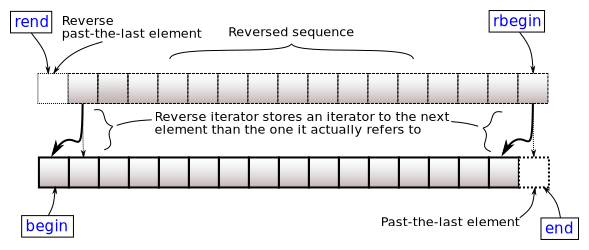
\includegraphics{resources/range-rbegin-rend.png}

\begin{itemize}
\tightlist
\item
  \textbf{begin( )} - returns iterator to the first element
\item
  \textbf{end( )} - returns iterator to the end (past the last element)
\item
  \textbf{rbegin( )} - returns reverse iterator to the last element
\item
  \textbf{rend( )} - returns a reverse iterator to the beginning (prior
  to the first element)
\end{itemize}

    \begin{tcolorbox}[breakable, size=fbox, boxrule=1pt, pad at break*=1mm,colback=cellbackground, colframe=cellborder]
\prompt{In}{incolor}{37}{\boxspacing}
\begin{Verbatim}[commandchars=\\\{\}]
\PY{c+c1}{// let\PYZsq{}s use iterator to traverse vectors}
\PY{c+c1}{// very similar to using for loop with index}
\PY{k}{for}\PY{p}{(}\PY{k}{auto} \PY{n}{iter} \PY{o}{=} \PY{n}{words}\PY{p}{.}\PY{n}{begin}\PY{p}{(}\PY{p}{)}\PY{p}{;} \PY{n}{iter} \PY{o}{!}\PY{o}{=} \PY{n}{words}\PY{p}{.}\PY{n}{end}\PY{p}{(}\PY{p}{)}\PY{p}{;} \PY{n}{iter}\PY{o}{+}\PY{o}{+}\PY{p}{)}
    \PY{n}{cout} \PY{o}{\PYZlt{}}\PY{o}{\PYZlt{}} \PY{o}{*}\PY{n}{iter} \PY{o}{\PYZlt{}}\PY{o}{\PYZlt{}} \PY{l+s}{\PYZdq{}}\PY{l+s}{; }\PY{l+s}{\PYZdq{}}\PY{p}{;} \PY{c+c1}{// iter is a pointer; so must derefernce to access value pointed to by iter}
\end{Verbatim}
\end{tcolorbox}

    \begin{Verbatim}[commandchars=\\\{\}]
I; love; c++; vectors;
    \end{Verbatim}

    \begin{tcolorbox}[breakable, size=fbox, boxrule=1pt, pad at break*=1mm,colback=cellbackground, colframe=cellborder]
\prompt{In}{incolor}{38}{\boxspacing}
\begin{Verbatim}[commandchars=\\\{\}]
\PY{c+c1}{// let\PYZsq{}s reverse traverse}
\PY{k}{for}\PY{p}{(}\PY{k}{auto} \PY{n}{iter} \PY{o}{=} \PY{n}{words}\PY{p}{.}\PY{n}{rbegin}\PY{p}{(}\PY{p}{)}\PY{p}{;} \PY{n}{iter} \PY{o}{!}\PY{o}{=} \PY{n}{words}\PY{p}{.}\PY{n}{rend}\PY{p}{(}\PY{p}{)}\PY{p}{;} \PY{n}{iter}\PY{o}{+}\PY{o}{+}\PY{p}{)}
    \PY{n}{cout} \PY{o}{\PYZlt{}}\PY{o}{\PYZlt{}} \PY{o}{*}\PY{n}{iter} \PY{o}{\PYZlt{}}\PY{o}{\PYZlt{}} \PY{l+s}{\PYZdq{}}\PY{l+s}{; }\PY{l+s}{\PYZdq{}}\PY{p}{;} \PY{c+c1}{// iter is a pointer; so must derefernce to access value pointed to by iter}
\end{Verbatim}
\end{tcolorbox}

    \begin{Verbatim}[commandchars=\\\{\}]
vectors; c++; love; I;
    \end{Verbatim}

    \hypertarget{aggregagte-operations}{%
\subsection{Aggregagte operations}\label{aggregagte-operations}}

\begin{itemize}
\tightlist
\item
  some aggegate operators such as assignment (=) and comparison
  (\textgreater, ==, etc.) are overloaded and work out of the box on
  vector objects as a whole
\item
  sorta works! - depends on what type of vector and if there's a
  predfined ordering of values in that type for sorting!
\item
  input, output (\texttt{\textless{}\textless{}},
  \texttt{\textgreater{}\textgreater{}}) operators do not work on vector
  objects as a whole
\end{itemize}

    \begin{tcolorbox}[breakable, size=fbox, boxrule=1pt, pad at break*=1mm,colback=cellbackground, colframe=cellborder]
\prompt{In}{incolor}{39}{\boxspacing}
\begin{Verbatim}[commandchars=\\\{\}]
\PY{c+c1}{// create words\PYZus{}copy vector with copy assignment}
\PY{n}{vector}\PY{o}{\PYZlt{}}\PY{n}{string}\PY{o}{\PYZgt{}} \PY{n}{words\PYZus{}copy} \PY{o}{=} \PY{n}{words}\PY{p}{;} \PY{c+c1}{// deep copies words into words\PYZus{}copy}
\end{Verbatim}
\end{tcolorbox}

    \begin{tcolorbox}[breakable, size=fbox, boxrule=1pt, pad at break*=1mm,colback=cellbackground, colframe=cellborder]
\prompt{In}{incolor}{42}{\boxspacing}
\begin{Verbatim}[commandchars=\\\{\}]
\PY{c+c1}{// string can be compared out of the box}
\PY{k}{if} \PY{p}{(}\PY{n}{words} \PY{o}{=}\PY{o}{=} \PY{n}{words\PYZus{}copy}\PY{p}{)}
    \PY{n}{cout} \PY{o}{\PYZlt{}}\PY{o}{\PYZlt{}} \PY{l+s}{\PYZdq{}}\PY{l+s}{two vectors are equal!}\PY{l+s}{\PYZdq{}}\PY{p}{;}
\PY{k}{else}
    \PY{n}{cout} \PY{o}{\PYZlt{}}\PY{o}{\PYZlt{}} \PY{l+s}{\PYZdq{}}\PY{l+s}{two vectors are not equal!}\PY{l+s}{\PYZdq{}}\PY{p}{;}
\end{Verbatim}
\end{tcolorbox}

    \begin{Verbatim}[commandchars=\\\{\}]
two vectors are equal!
    \end{Verbatim}

    \hypertarget{passing-vectors-to-functions}{%
\subsection{Passing vectors to
functions}\label{passing-vectors-to-functions}}

\begin{itemize}
\tightlist
\item
  vector can be passed to functions by value or by reference
\item
  unless required, it's always efficient to pass containers type such as
  vectors to function by reference

  \begin{itemize}
  \tightlist
  \item
    copying data can be costly (can take a long time) depending on the
    amount of data vector is storing
  \end{itemize}
\end{itemize}

    \begin{tcolorbox}[breakable, size=fbox, boxrule=1pt, pad at break*=1mm,colback=cellbackground, colframe=cellborder]
\prompt{In}{incolor}{44}{\boxspacing}
\begin{Verbatim}[commandchars=\\\{\}]
\PY{c+c1}{// given a vector of values find and return average }
\PY{k+kt}{float} \PY{n+nf}{findAverage}\PY{p}{(}\PY{k}{const} \PY{n}{vector}\PY{o}{\PYZlt{}}\PY{k+kt}{int}\PY{o}{\PYZgt{}} \PY{o}{\PYZam{}} \PY{n}{v}\PY{p}{)} \PY{p}{\PYZob{}}
    \PY{k+kt}{float} \PY{n}{sum} \PY{o}{=} \PY{l+m+mi}{0}\PY{p}{;}
    \PY{k}{for} \PY{p}{(}\PY{k}{auto} \PY{n+nl}{val}\PY{p}{:} \PY{n}{v}\PY{p}{)}
        \PY{n}{sum} \PY{o}{+}\PY{o}{=} \PY{n}{val}\PY{p}{;}
    \PY{k}{return} \PY{n}{sum}\PY{o}{/}\PY{n}{v}\PY{p}{.}\PY{n}{size}\PY{p}{(}\PY{p}{)}\PY{p}{;}
\PY{p}{\PYZcb{}}
\end{Verbatim}
\end{tcolorbox}

    \begin{tcolorbox}[breakable, size=fbox, boxrule=1pt, pad at break*=1mm,colback=cellbackground, colframe=cellborder]
\prompt{In}{incolor}{45}{\boxspacing}
\begin{Verbatim}[commandchars=\\\{\}]
\PY{c+c1}{// let\PYZsq{}s see the values of age vector}
\PY{n}{age}
\end{Verbatim}
\end{tcolorbox}

            \begin{tcolorbox}[breakable, size=fbox, boxrule=.5pt, pad at break*=1mm, opacityfill=0]
\prompt{Out}{outcolor}{45}{\boxspacing}
\begin{Verbatim}[commandchars=\\\{\}]
\{ 25, 39 \}
\end{Verbatim}
\end{tcolorbox}
        
    \begin{tcolorbox}[breakable, size=fbox, boxrule=1pt, pad at break*=1mm,colback=cellbackground, colframe=cellborder]
\prompt{In}{incolor}{46}{\boxspacing}
\begin{Verbatim}[commandchars=\\\{\}]
\PY{n}{cout} \PY{o}{\PYZlt{}}\PY{o}{\PYZlt{}} \PY{l+s}{\PYZdq{}}\PY{l+s}{average age = }\PY{l+s}{\PYZdq{}} \PY{o}{\PYZlt{}}\PY{o}{\PYZlt{}} \PY{n}{findAverage}\PY{p}{(}\PY{n}{age}\PY{p}{)}\PY{p}{;}
\end{Verbatim}
\end{tcolorbox}

    \begin{Verbatim}[commandchars=\\\{\}]
average age = 32
    \end{Verbatim}

    \begin{tcolorbox}[breakable, size=fbox, boxrule=1pt, pad at break*=1mm,colback=cellbackground, colframe=cellborder]
\prompt{In}{incolor}{47}{\boxspacing}
\begin{Verbatim}[commandchars=\\\{\}]
\PY{c+c1}{// printVector function}
\PY{k}{template}\PY{o}{\PYZlt{}}\PY{k}{class} \PY{n+nc}{T}\PY{o}{\PYZgt{}}
\PY{k+kt}{void} \PY{n}{printVector}\PY{p}{(}\PY{k}{const} \PY{n}{vector}\PY{o}{\PYZlt{}}\PY{n}{T}\PY{o}{\PYZgt{}}\PY{o}{\PYZam{}} \PY{n}{v}\PY{p}{)} \PY{p}{\PYZob{}}
    \PY{k+kt}{char} \PY{n}{comma}\PY{p}{[}\PY{l+m+mi}{3}\PY{p}{]} \PY{o}{=} \PY{p}{\PYZob{}}\PY{l+s+sc}{\PYZsq{}}\PY{l+s+sc}{\PYZbs{}0}\PY{l+s+sc}{\PYZsq{}}\PY{p}{,} \PY{l+s+sc}{\PYZsq{}}\PY{l+s+sc}{ }\PY{l+s+sc}{\PYZsq{}}\PY{p}{,} \PY{l+s+sc}{\PYZsq{}}\PY{l+s+sc}{\PYZbs{}0}\PY{l+s+sc}{\PYZsq{}}\PY{p}{\PYZcb{}}\PY{p}{;}
    \PY{n}{cout} \PY{o}{\PYZlt{}}\PY{o}{\PYZlt{}} \PY{l+s+sc}{\PYZsq{}}\PY{l+s+sc}{[}\PY{l+s+sc}{\PYZsq{}}\PY{p}{;}
    \PY{k}{for} \PY{p}{(}\PY{k}{const} \PY{k}{auto}\PY{o}{\PYZam{}} \PY{n+nl}{e}\PY{p}{:} \PY{n}{v}\PY{p}{)} \PY{p}{\PYZob{}}
        \PY{n}{cout} \PY{o}{\PYZlt{}}\PY{o}{\PYZlt{}} \PY{n}{comma} \PY{o}{\PYZlt{}}\PY{o}{\PYZlt{}} \PY{n}{e}\PY{p}{;}
        \PY{n}{comma}\PY{p}{[}\PY{l+m+mi}{0}\PY{p}{]} \PY{o}{=} \PY{l+s+sc}{\PYZsq{}}\PY{l+s+sc}{,}\PY{l+s+sc}{\PYZsq{}}\PY{p}{;}
    \PY{p}{\PYZcb{}}
    \PY{n}{cout} \PY{o}{\PYZlt{}}\PY{o}{\PYZlt{}} \PY{l+s}{\PYZdq{}}\PY{l+s}{]}\PY{l+s+se}{\PYZbs{}n}\PY{l+s}{\PYZdq{}}\PY{p}{;}
\PY{p}{\PYZcb{}}
\end{Verbatim}
\end{tcolorbox}

    \begin{tcolorbox}[breakable, size=fbox, boxrule=1pt, pad at break*=1mm,colback=cellbackground, colframe=cellborder]
\prompt{In}{incolor}{48}{\boxspacing}
\begin{Verbatim}[commandchars=\\\{\}]
\PY{n}{printVector}\PY{p}{(}\PY{n}{words}\PY{p}{)}\PY{p}{;}
\end{Verbatim}
\end{tcolorbox}

    \begin{Verbatim}[commandchars=\\\{\}]
[I, love, c++, vectors]
    \end{Verbatim}

    \begin{tcolorbox}[breakable, size=fbox, boxrule=1pt, pad at break*=1mm,colback=cellbackground, colframe=cellborder]
\prompt{In}{incolor}{49}{\boxspacing}
\begin{Verbatim}[commandchars=\\\{\}]
\PY{n}{printVector}\PY{p}{(}\PY{n}{age}\PY{p}{)}
\end{Verbatim}
\end{tcolorbox}

    \begin{Verbatim}[commandchars=\\\{\}]
[25, 39]
    \end{Verbatim}

    \hypertarget{returning-vector-from-functions}{%
\subsection{Returning vector from
functions}\label{returning-vector-from-functions}}

\begin{itemize}
\tightlist
\item
  since vector supports \texttt{=} copy operator, returning vector from
  functions is possible
\item
  since returned vector needs to be copied it can be costly

  \begin{itemize}
  \tightlist
  \item
    it's best practice to pass vector as reference to get the
    data/results out of functions
  \end{itemize}
\end{itemize}

    \begin{tcolorbox}[breakable, size=fbox, boxrule=1pt, pad at break*=1mm,colback=cellbackground, colframe=cellborder]
\prompt{In}{incolor}{8}{\boxspacing}
\begin{Verbatim}[commandchars=\\\{\}]
\PY{c+c1}{// function that gets vector of integers from standard input}
\PY{k+kt}{void} \PY{n+nf}{getNumbers}\PY{p}{(}\PY{n}{vector}\PY{o}{\PYZlt{}}\PY{k+kt}{int}\PY{o}{\PYZgt{}} \PY{o}{\PYZam{}} \PY{n}{numbers}\PY{p}{)} \PY{p}{\PYZob{}}
    \PY{n}{cout} \PY{o}{\PYZlt{}}\PY{o}{\PYZlt{}} \PY{l+s}{\PYZdq{}}\PY{l+s}{Enter as many whole numbers as you wish.}\PY{l+s+se}{\PYZbs{}n}\PY{l+s}{Enter \PYZsq{}done\PYZsq{} when done:}\PY{l+s+se}{\PYZbs{}n}\PY{l+s}{\PYZdq{}}\PY{p}{;}
    \PY{k+kt}{int} \PY{n}{num}\PY{p}{;}
    \PY{k}{while}\PY{p}{(}\PY{n}{cin} \PY{o}{\PYZgt{}}\PY{o}{\PYZgt{}} \PY{n}{num}\PY{p}{)} \PY{c+c1}{// cin returns false when it fails to parse \PYZsq{}done\PYZsq{}}
        \PY{n}{numbers}\PY{p}{.}\PY{n}{push\PYZus{}back}\PY{p}{(}\PY{n}{num}\PY{p}{)}\PY{p}{;}
\PY{p}{\PYZcb{}}
\end{Verbatim}
\end{tcolorbox}

    \begin{tcolorbox}[breakable, size=fbox, boxrule=1pt, pad at break*=1mm,colback=cellbackground, colframe=cellborder]
\prompt{In}{incolor}{9}{\boxspacing}
\begin{Verbatim}[commandchars=\\\{\}]
\PY{c+c1}{// create an empty vector}
\PY{n}{vector}\PY{o}{\PYZlt{}}\PY{k+kt}{int}\PY{o}{\PYZgt{}} \PY{n}{my\PYZus{}numbers}\PY{p}{;}
\end{Verbatim}
\end{tcolorbox}

    \begin{tcolorbox}[breakable, size=fbox, boxrule=1pt, pad at break*=1mm,colback=cellbackground, colframe=cellborder]
\prompt{In}{incolor}{10}{\boxspacing}
\begin{Verbatim}[commandchars=\\\{\}]
\PY{n}{getNumbers}\PY{p}{(}\PY{n}{my\PYZus{}numbers}\PY{p}{)}\PY{p}{;}
\end{Verbatim}
\end{tcolorbox}

    \begin{Verbatim}[commandchars=\\\{\}]
Enter as many whole numbers as you wish.
Enter 'done' when done:
10
19
100
345
56
45
66
999
4546
done
    \end{Verbatim}

    \begin{tcolorbox}[breakable, size=fbox, boxrule=1pt, pad at break*=1mm,colback=cellbackground, colframe=cellborder]
\prompt{In}{incolor}{11}{\boxspacing}
\begin{Verbatim}[commandchars=\\\{\}]
\PY{n}{my\PYZus{}numbers}
\end{Verbatim}
\end{tcolorbox}

            \begin{tcolorbox}[breakable, size=fbox, boxrule=.5pt, pad at break*=1mm, opacityfill=0]
\prompt{Out}{outcolor}{11}{\boxspacing}
\begin{Verbatim}[commandchars=\\\{\}]
\{ 10, 19, 100, 345, 56, 45, 66, 999, 4546 \}
\end{Verbatim}
\end{tcolorbox}
        
    \hypertarget{two-dimensional-vector}{%
\subsection{Two-dimensional vector}\label{two-dimensional-vector}}

\begin{itemize}
\tightlist
\item
  if we insert vectors as an element to a vector, we essentially get a
  2-D vector

  \begin{itemize}
  \tightlist
  \item
    works similar to 2-D array
  \end{itemize}
\end{itemize}

    \begin{tcolorbox}[breakable, size=fbox, boxrule=1pt, pad at break*=1mm,colback=cellbackground, colframe=cellborder]
\prompt{In}{incolor}{10}{\boxspacing}
\begin{Verbatim}[commandchars=\\\{\}]
\PY{c+c1}{// let\PYZsq{}s declare a 2\PYZhy{}d vector of integers}
\PY{n}{vector}\PY{o}{\PYZlt{}} \PY{n}{vector}\PY{o}{\PYZlt{}}\PY{k+kt}{int}\PY{o}{\PYZgt{}} \PY{o}{\PYZgt{}} \PY{n}{matrix}\PY{p}{;}
\end{Verbatim}
\end{tcolorbox}

    \begin{tcolorbox}[breakable, size=fbox, boxrule=1pt, pad at break*=1mm,colback=cellbackground, colframe=cellborder]
\prompt{In}{incolor}{11}{\boxspacing}
\begin{Verbatim}[commandchars=\\\{\}]
\PY{c+c1}{// add the first vector \PYZhy{} first row}
\PY{n}{matrix}\PY{p}{.}\PY{n}{push\PYZus{}back}\PY{p}{(}\PY{p}{\PYZob{}}\PY{l+m+mi}{1}\PY{p}{,} \PY{l+m+mi}{2}\PY{p}{,} \PY{l+m+mi}{3}\PY{p}{,} \PY{l+m+mi}{4}\PY{p}{\PYZcb{}}\PY{p}{)}\PY{p}{;}
\end{Verbatim}
\end{tcolorbox}

    \begin{tcolorbox}[breakable, size=fbox, boxrule=1pt, pad at break*=1mm,colback=cellbackground, colframe=cellborder]
\prompt{In}{incolor}{12}{\boxspacing}
\begin{Verbatim}[commandchars=\\\{\}]
\PY{n}{matrix}\PY{p}{[}\PY{l+m+mi}{0}\PY{p}{]}
\end{Verbatim}
\end{tcolorbox}

            \begin{tcolorbox}[breakable, size=fbox, boxrule=.5pt, pad at break*=1mm, opacityfill=0]
\prompt{Out}{outcolor}{12}{\boxspacing}
\begin{Verbatim}[commandchars=\\\{\}]
\{ 1, 2, 3, 4 \}
\end{Verbatim}
\end{tcolorbox}
        
    \begin{tcolorbox}[breakable, size=fbox, boxrule=1pt, pad at break*=1mm,colback=cellbackground, colframe=cellborder]
\prompt{In}{incolor}{13}{\boxspacing}
\begin{Verbatim}[commandchars=\\\{\}]
\PY{c+c1}{// let\PYZsq{}s add an empty vector as the second element or 2nd row}
\PY{n}{matrix}\PY{p}{.}\PY{n}{push\PYZus{}back}\PY{p}{(}\PY{n}{vector}\PY{o}{\PYZlt{}}\PY{k+kt}{int}\PY{o}{\PYZgt{}}\PY{p}{(}\PY{p}{)}\PY{p}{)}\PY{p}{;}
\end{Verbatim}
\end{tcolorbox}

    \begin{tcolorbox}[breakable, size=fbox, boxrule=1pt, pad at break*=1mm,colback=cellbackground, colframe=cellborder]
\prompt{In}{incolor}{14}{\boxspacing}
\begin{Verbatim}[commandchars=\\\{\}]
\PY{c+c1}{// let\PYZsq{}s add elements to the 2nd vector or 2nd row}
\PY{n}{matrix}\PY{p}{[}\PY{l+m+mi}{1}\PY{p}{]}\PY{p}{.}\PY{n}{push\PYZus{}back}\PY{p}{(}\PY{l+m+mi}{5}\PY{p}{)}\PY{p}{;}
\PY{n}{matrix}\PY{p}{[}\PY{l+m+mi}{1}\PY{p}{]}\PY{p}{.}\PY{n}{push\PYZus{}back}\PY{p}{(}\PY{l+m+mi}{6}\PY{p}{)}\PY{p}{;}
\PY{n}{matrix}\PY{p}{[}\PY{l+m+mi}{1}\PY{p}{]}\PY{p}{.}\PY{n}{push\PYZus{}back}\PY{p}{(}\PY{l+m+mi}{7}\PY{p}{)}\PY{p}{;}
\PY{n}{matrix}\PY{p}{[}\PY{l+m+mi}{1}\PY{p}{]}\PY{p}{.}\PY{n}{push\PYZus{}back}\PY{p}{(}\PY{l+m+mi}{8}\PY{p}{)}\PY{p}{;}
\end{Verbatim}
\end{tcolorbox}

    \begin{tcolorbox}[breakable, size=fbox, boxrule=1pt, pad at break*=1mm,colback=cellbackground, colframe=cellborder]
\prompt{In}{incolor}{15}{\boxspacing}
\begin{Verbatim}[commandchars=\\\{\}]
\PY{n}{matrix}\PY{p}{[}\PY{l+m+mi}{1}\PY{p}{]}
\end{Verbatim}
\end{tcolorbox}

            \begin{tcolorbox}[breakable, size=fbox, boxrule=.5pt, pad at break*=1mm, opacityfill=0]
\prompt{Out}{outcolor}{15}{\boxspacing}
\begin{Verbatim}[commandchars=\\\{\}]
\{ 5, 6, 7, 8 \}
\end{Verbatim}
\end{tcolorbox}
        
    \begin{tcolorbox}[breakable, size=fbox, boxrule=1pt, pad at break*=1mm,colback=cellbackground, colframe=cellborder]
\prompt{In}{incolor}{16}{\boxspacing}
\begin{Verbatim}[commandchars=\\\{\}]
\PY{c+c1}{// access element of vector elements}
\PY{c+c1}{// first row, first column}
\PY{n}{matrix}\PY{p}{[}\PY{l+m+mi}{0}\PY{p}{]}\PY{p}{[}\PY{l+m+mi}{0}\PY{p}{]}
\end{Verbatim}
\end{tcolorbox}

            \begin{tcolorbox}[breakable, size=fbox, boxrule=.5pt, pad at break*=1mm, opacityfill=0]
\prompt{Out}{outcolor}{16}{\boxspacing}
\begin{Verbatim}[commandchars=\\\{\}]
1
\end{Verbatim}
\end{tcolorbox}
        
    \begin{tcolorbox}[breakable, size=fbox, boxrule=1pt, pad at break*=1mm,colback=cellbackground, colframe=cellborder]
\prompt{In}{incolor}{17}{\boxspacing}
\begin{Verbatim}[commandchars=\\\{\}]
\PY{c+c1}{// 2nd row, fourth column}
\PY{n}{matrix}\PY{p}{[}\PY{l+m+mi}{1}\PY{p}{]}\PY{p}{[}\PY{l+m+mi}{3}\PY{p}{]}
\end{Verbatim}
\end{tcolorbox}

            \begin{tcolorbox}[breakable, size=fbox, boxrule=.5pt, pad at break*=1mm, opacityfill=0]
\prompt{Out}{outcolor}{17}{\boxspacing}
\begin{Verbatim}[commandchars=\\\{\}]
8
\end{Verbatim}
\end{tcolorbox}
        
    \hypertarget{sort-vector}{%
\subsection{Sort vector}\label{sort-vector}}

\begin{itemize}
\tightlist
\item
  vector like array needs to be sorted often to solve many problems
\item
  let's use built-in \texttt{sort} function in \texttt{algorithm}
  library

  \begin{itemize}
  \tightlist
  \item
    \texttt{sort} function implements one of the fastest sorting
    algorithms
  \end{itemize}
\end{itemize}

    \begin{tcolorbox}[breakable, size=fbox, boxrule=1pt, pad at break*=1mm,colback=cellbackground, colframe=cellborder]
\prompt{In}{incolor}{2}{\boxspacing}
\begin{Verbatim}[commandchars=\\\{\}]
\PY{c+cp}{\PYZsh{}}\PY{c+cp}{include} \PY{c+cpf}{\PYZlt{}vector\PYZgt{}}
\PY{c+cp}{\PYZsh{}}\PY{c+cp}{include} \PY{c+cpf}{\PYZlt{}algorithm\PYZgt{}}\PY{c+c1}{ // sort()}
\PY{c+cp}{\PYZsh{}}\PY{c+cp}{include} \PY{c+cpf}{\PYZlt{}iterator\PYZgt{}}\PY{c+c1}{ // begin() and end()}
\PY{c+cp}{\PYZsh{}}\PY{c+cp}{include} \PY{c+cpf}{\PYZlt{}functional\PYZgt{}}\PY{c+c1}{ // greater\PYZlt{}\PYZgt{}();}
\PY{c+cp}{\PYZsh{}}\PY{c+cp}{include} \PY{c+cpf}{\PYZlt{}iostream\PYZgt{}}

\PY{k}{using} \PY{k}{namespace} \PY{n+nn}{std}\PY{p}{;}
\end{Verbatim}
\end{tcolorbox}

    \begin{tcolorbox}[breakable, size=fbox, boxrule=1pt, pad at break*=1mm,colback=cellbackground, colframe=cellborder]
\prompt{In}{incolor}{3}{\boxspacing}
\begin{Verbatim}[commandchars=\\\{\}]
\PY{n}{vector}\PY{o}{\PYZlt{}}\PY{k+kt}{int}\PY{o}{\PYZgt{}} \PY{n}{some\PYZus{}values} \PY{o}{=} \PY{p}{\PYZob{}} \PY{l+m+mi}{100}\PY{p}{,} \PY{l+m+mi}{99}\PY{p}{,} \PY{l+m+mi}{85}\PY{p}{,} \PY{l+m+mi}{40}\PY{p}{,} \PY{l+m+mi}{1233}\PY{p}{,} \PY{l+m+mi}{1}\PY{p}{\PYZcb{}}\PY{p}{;}
\end{Verbatim}
\end{tcolorbox}

    \begin{tcolorbox}[breakable, size=fbox, boxrule=1pt, pad at break*=1mm,colback=cellbackground, colframe=cellborder]
\prompt{In}{incolor}{7}{\boxspacing}
\begin{Verbatim}[commandchars=\\\{\}]
\PY{c+c1}{// let\PYZsq{}s sort some\PYZus{}values }
\PY{n}{sort}\PY{p}{(}\PY{n}{begin}\PY{p}{(}\PY{n}{some\PYZus{}values}\PY{p}{)}\PY{p}{,} \PY{n}{end}\PY{p}{(}\PY{n}{some\PYZus{}values}\PY{p}{)}\PY{p}{)}\PY{p}{;}
\end{Verbatim}
\end{tcolorbox}

    \begin{tcolorbox}[breakable, size=fbox, boxrule=1pt, pad at break*=1mm,colback=cellbackground, colframe=cellborder]
\prompt{In}{incolor}{8}{\boxspacing}
\begin{Verbatim}[commandchars=\\\{\}]
\PY{n}{some\PYZus{}values}
\end{Verbatim}
\end{tcolorbox}

            \begin{tcolorbox}[breakable, size=fbox, boxrule=.5pt, pad at break*=1mm, opacityfill=0]
\prompt{Out}{outcolor}{8}{\boxspacing}
\begin{Verbatim}[commandchars=\\\{\}]
\{ 1, 40, 85, 99, 100, 1233 \}
\end{Verbatim}
\end{tcolorbox}
        
    \begin{tcolorbox}[breakable, size=fbox, boxrule=1pt, pad at break*=1mm,colback=cellbackground, colframe=cellborder]
\prompt{In}{incolor}{18}{\boxspacing}
\begin{Verbatim}[commandchars=\\\{\}]
\PY{c+c1}{// let\PYZsq{}s sort 1st row of matrix in reverse order}
\PY{n}{matrix}\PY{p}{[}\PY{l+m+mi}{0}\PY{p}{]}
\end{Verbatim}
\end{tcolorbox}

            \begin{tcolorbox}[breakable, size=fbox, boxrule=.5pt, pad at break*=1mm, opacityfill=0]
\prompt{Out}{outcolor}{18}{\boxspacing}
\begin{Verbatim}[commandchars=\\\{\}]
\{ 1, 2, 3, 4 \}
\end{Verbatim}
\end{tcolorbox}
        
    \begin{tcolorbox}[breakable, size=fbox, boxrule=1pt, pad at break*=1mm,colback=cellbackground, colframe=cellborder]
\prompt{In}{incolor}{19}{\boxspacing}
\begin{Verbatim}[commandchars=\\\{\}]
\PY{c+c1}{// sort in increasing order}
\PY{n}{sort}\PY{p}{(}\PY{n}{matrix}\PY{p}{[}\PY{l+m+mi}{0}\PY{p}{]}\PY{p}{.}\PY{n}{begin}\PY{p}{(}\PY{p}{)}\PY{p}{,} \PY{n}{matrix}\PY{p}{[}\PY{l+m+mi}{0}\PY{p}{]}\PY{p}{.}\PY{n}{end}\PY{p}{(}\PY{p}{)}\PY{p}{)}\PY{p}{;}
\end{Verbatim}
\end{tcolorbox}

    \begin{tcolorbox}[breakable, size=fbox, boxrule=1pt, pad at break*=1mm,colback=cellbackground, colframe=cellborder]
\prompt{In}{incolor}{20}{\boxspacing}
\begin{Verbatim}[commandchars=\\\{\}]
\PY{n}{matrix}\PY{p}{[}\PY{l+m+mi}{0}\PY{p}{]}
\end{Verbatim}
\end{tcolorbox}

            \begin{tcolorbox}[breakable, size=fbox, boxrule=.5pt, pad at break*=1mm, opacityfill=0]
\prompt{Out}{outcolor}{20}{\boxspacing}
\begin{Verbatim}[commandchars=\\\{\}]
\{ 1, 2, 3, 4 \}
\end{Verbatim}
\end{tcolorbox}
        
    \begin{tcolorbox}[breakable, size=fbox, boxrule=1pt, pad at break*=1mm,colback=cellbackground, colframe=cellborder]
\prompt{In}{incolor}{21}{\boxspacing}
\begin{Verbatim}[commandchars=\\\{\}]
\PY{c+c1}{// sort in on\PYZhy{}increasing order}
\PY{n}{sort}\PY{p}{(}\PY{n}{matrix}\PY{p}{[}\PY{l+m+mi}{0}\PY{p}{]}\PY{p}{.}\PY{n}{begin}\PY{p}{(}\PY{p}{)}\PY{p}{,} \PY{n}{matrix}\PY{p}{[}\PY{l+m+mi}{0}\PY{p}{]}\PY{p}{.}\PY{n}{end}\PY{p}{(}\PY{p}{)}\PY{p}{,} \PY{n}{greater}\PY{o}{\PYZlt{}}\PY{k+kt}{int}\PY{o}{\PYZgt{}}\PY{p}{(}\PY{p}{)}\PY{p}{)}\PY{p}{;}
\end{Verbatim}
\end{tcolorbox}

    \begin{tcolorbox}[breakable, size=fbox, boxrule=1pt, pad at break*=1mm,colback=cellbackground, colframe=cellborder]
\prompt{In}{incolor}{22}{\boxspacing}
\begin{Verbatim}[commandchars=\\\{\}]
\PY{n}{matrix}\PY{p}{[}\PY{l+m+mi}{0}\PY{p}{]}
\end{Verbatim}
\end{tcolorbox}

            \begin{tcolorbox}[breakable, size=fbox, boxrule=.5pt, pad at break*=1mm, opacityfill=0]
\prompt{Out}{outcolor}{22}{\boxspacing}
\begin{Verbatim}[commandchars=\\\{\}]
\{ 4, 3, 2, 1 \}
\end{Verbatim}
\end{tcolorbox}
        
    \hypertarget{labs}{%
\subsection{Labs}\label{labs}}

\begin{enumerate}
\def\labelenumi{\arabic{enumi}.}
\tightlist
\item
  The following lab demonstrates the usage of vector data structure and
  some operations on vectors.

  \begin{itemize}
  \tightlist
  \item
    use partial solution \texttt{numberSystem.cpp} file in
    \href{./labs/vectors/}{labs/vectors/} folder
  \item
    use Makefile to compile and debug the program
  \item
    fixe all the FIXMEs and write \#FIXED\# next to each FIXME once
    fixed
  \end{itemize}
\end{enumerate}

    \hypertarget{exercises}{%
\subsection{Exercises}\label{exercises}}

\hypertarget{sove-all-exercises-listed-in-array-chapter-using-vector-instead.}{%
\subsubsection{Sove all exercises listed in Array chapter using vector
instead.}\label{sove-all-exercises-listed-in-array-chapter-using-vector-instead.}}

\hypertarget{more-exercises}{%
\subsubsection{More exercises}\label{more-exercises}}

\begin{enumerate}
\def\labelenumi{\arabic{enumi}.}
\tightlist
\item
  Write a function that splits a given text/string into a vector of
  individual words

  \begin{itemize}
  \tightlist
  \item
    each word is sequence of characters separated by a whitespace
  \item
    write 3 test cases
  \end{itemize}
\end{enumerate}

    \begin{tcolorbox}[breakable, size=fbox, boxrule=1pt, pad at break*=1mm,colback=cellbackground, colframe=cellborder]
\prompt{In}{incolor}{23}{\boxspacing}
\begin{Verbatim}[commandchars=\\\{\}]
\PY{c+c1}{// Solution to Exercise 1}
\PY{k+kt}{void} \PY{n+nf}{splitString}\PY{p}{(}\PY{n}{vector}\PY{o}{\PYZlt{}}\PY{n}{string}\PY{o}{\PYZgt{}} \PY{o}{\PYZam{}}\PY{n}{words}\PY{p}{,} \PY{n}{string} \PY{n}{text}\PY{p}{)} \PY{p}{\PYZob{}}
    \PY{n}{string} \PY{n}{word}\PY{p}{;}
    \PY{n}{stringstream} \PY{n}{ss}\PY{p}{(}\PY{n}{text}\PY{p}{)}\PY{p}{;}
    \PY{k}{while} \PY{p}{(}\PY{n}{ss} \PY{o}{\PYZgt{}}\PY{o}{\PYZgt{}} \PY{n}{word}\PY{p}{)} \PY{p}{\PYZob{}}
        \PY{n}{words}\PY{p}{.}\PY{n}{push\PYZus{}back}\PY{p}{(}\PY{n}{word}\PY{p}{)}\PY{p}{;}
    \PY{p}{\PYZcb{}}
\PY{p}{\PYZcb{}}
\end{Verbatim}
\end{tcolorbox}

    \begin{tcolorbox}[breakable, size=fbox, boxrule=1pt, pad at break*=1mm,colback=cellbackground, colframe=cellborder]
\prompt{In}{incolor}{24}{\boxspacing}
\begin{Verbatim}[commandchars=\\\{\}]
\PY{k+kt}{void} \PY{n+nf}{test\PYZus{}splitString}\PY{p}{(}\PY{p}{)} \PY{p}{\PYZob{}}
    \PY{n}{vector}\PY{o}{\PYZlt{}}\PY{n}{string}\PY{o}{\PYZgt{}} \PY{n}{answer}\PY{p}{;}
    \PY{n}{splitString}\PY{p}{(}\PY{n}{answer}\PY{p}{,} \PY{l+s}{\PYZdq{}}\PY{l+s}{word}\PY{l+s}{\PYZdq{}}\PY{p}{)}\PY{p}{;}
    \PY{n}{vector}\PY{o}{\PYZlt{}}\PY{n}{string}\PY{o}{\PYZgt{}} \PY{n}{actual} \PY{o}{=} \PY{p}{\PYZob{}}\PY{l+s}{\PYZdq{}}\PY{l+s}{word}\PY{l+s}{\PYZdq{}}\PY{p}{\PYZcb{}}\PY{p}{;}
    \PY{n}{assert}\PY{p}{(}\PY{n}{answer} \PY{o}{=}\PY{o}{=} \PY{n}{actual}\PY{p}{)}\PY{p}{;}
    \PY{n}{answer}\PY{p}{.}\PY{n}{clear}\PY{p}{(}\PY{p}{)}\PY{p}{;}
    \PY{n}{splitString}\PY{p}{(}\PY{n}{answer}\PY{p}{,} \PY{l+s}{\PYZdq{}}\PY{l+s}{two word}\PY{l+s}{\PYZdq{}}\PY{p}{)}\PY{p}{;}
    \PY{n}{vector}\PY{o}{\PYZlt{}}\PY{n}{string}\PY{o}{\PYZgt{}} \PY{n}{actual1} \PY{o}{=} \PY{p}{\PYZob{}}\PY{l+s}{\PYZdq{}}\PY{l+s}{two, word}\PY{l+s}{\PYZdq{}}\PY{p}{\PYZcb{}}\PY{p}{;}
    \PY{n}{assert}\PY{p}{(}\PY{n}{answer} \PY{o}{=}\PY{o}{=} \PY{n}{actual1}\PY{p}{)}\PY{p}{;}
    \PY{n}{answer}\PY{p}{.}\PY{n}{clear}\PY{p}{(}\PY{p}{)}\PY{p}{;}
    \PY{n}{splitString}\PY{p}{(}\PY{n}{answer}\PY{p}{,} \PY{l+s}{\PYZdq{}}\PY{l+s}{A sentence with multiple words!}\PY{l+s}{\PYZdq{}}\PY{p}{)}\PY{p}{;}
    \PY{n}{vector}\PY{o}{\PYZlt{}}\PY{n}{string}\PY{o}{\PYZgt{}} \PY{n}{actual2} \PY{o}{=} \PY{p}{\PYZob{}}\PY{l+s}{\PYZdq{}}\PY{l+s}{A}\PY{l+s}{\PYZdq{}}\PY{p}{,} \PY{l+s}{\PYZdq{}}\PY{l+s}{sentence}\PY{l+s}{\PYZdq{}}\PY{p}{,} \PY{l+s}{\PYZdq{}}\PY{l+s}{with}\PY{l+s}{\PYZdq{}}\PY{p}{,} \PY{l+s}{\PYZdq{}}\PY{l+s}{multiple}\PY{l+s}{\PYZdq{}}\PY{p}{,} \PY{l+s}{\PYZdq{}}\PY{l+s}{words!}\PY{l+s}{\PYZdq{}}\PY{p}{\PYZcb{}}\PY{p}{;}
    \PY{n}{assert}\PY{p}{(}\PY{n}{answer} \PY{o}{=}\PY{o}{=} \PY{n}{actual2}\PY{p}{)}\PY{p}{;}
    \PY{n}{answer}\PY{p}{.}\PY{n}{clear}\PY{p}{(}\PY{p}{)}\PY{p}{;}
    \PY{n}{cerr} \PY{o}{\PYZlt{}}\PY{o}{\PYZlt{}} \PY{l+s}{\PYZdq{}}\PY{l+s}{all test cases is passed for splitString()}\PY{l+s+se}{\PYZbs{}n}\PY{l+s}{\PYZdq{}}\PY{p}{;}
\PY{p}{\PYZcb{}}
\end{Verbatim}
\end{tcolorbox}

    \begin{tcolorbox}[breakable, size=fbox, boxrule=1pt, pad at break*=1mm,colback=cellbackground, colframe=cellborder]
\prompt{In}{incolor}{25}{\boxspacing}
\begin{Verbatim}[commandchars=\\\{\}]
\PY{n}{test\PYZus{}splitString}\PY{p}{(}\PY{p}{)}\PY{p}{;}
\end{Verbatim}
\end{tcolorbox}

    \begin{Verbatim}[commandchars=\\\{\}]
all test cases is passed for splitString()
    \end{Verbatim}

    \begin{tcolorbox}[breakable, size=fbox, boxrule=1pt, pad at break*=1mm,colback=cellbackground, colframe=cellborder]
\prompt{In}{incolor}{26}{\boxspacing}
\begin{Verbatim}[commandchars=\\\{\}]
\PY{n}{vector}\PY{o}{\PYZlt{}}\PY{n}{string}\PY{o}{\PYZgt{}} \PY{n}{tokens}\PY{p}{;}
\end{Verbatim}
\end{tcolorbox}

    \begin{tcolorbox}[breakable, size=fbox, boxrule=1pt, pad at break*=1mm,colback=cellbackground, colframe=cellborder]
\prompt{In}{incolor}{27}{\boxspacing}
\begin{Verbatim}[commandchars=\\\{\}]
\PY{c+c1}{// not needed but just in case!}
\PY{n}{tokens}\PY{p}{.}\PY{n}{clear}\PY{p}{(}\PY{p}{)}\PY{p}{;}
\end{Verbatim}
\end{tcolorbox}

    \begin{tcolorbox}[breakable, size=fbox, boxrule=1pt, pad at break*=1mm,colback=cellbackground, colframe=cellborder]
\prompt{In}{incolor}{28}{\boxspacing}
\begin{Verbatim}[commandchars=\\\{\}]
\PY{n}{splitString}\PY{p}{(}\PY{n}{tokens}\PY{p}{,} \PY{l+s}{\PYZdq{}}\PY{l+s}{This is a long sentence so long that it\PYZsq{}s hard to comprehend!}\PY{l+s}{\PYZdq{}}\PY{p}{)}\PY{p}{;}
\end{Verbatim}
\end{tcolorbox}

    \begin{tcolorbox}[breakable, size=fbox, boxrule=1pt, pad at break*=1mm,colback=cellbackground, colframe=cellborder]
\prompt{In}{incolor}{29}{\boxspacing}
\begin{Verbatim}[commandchars=\\\{\}]
\PY{n}{tokens}
\end{Verbatim}
\end{tcolorbox}

            \begin{tcolorbox}[breakable, size=fbox, boxrule=.5pt, pad at break*=1mm, opacityfill=0]
\prompt{Out}{outcolor}{29}{\boxspacing}
\begin{Verbatim}[commandchars=\\\{\}]
\{ "This", "is", "a", "long", "sentence", "so", "long", "that", "it's", "hard",
"to", "comprehend!" \}
\end{Verbatim}
\end{tcolorbox}
        
    \hypertarget{complete-program-can-be-found-in-demosstringssplitstring}{%
\subsubsection{\texorpdfstring{complete program can be found in
\href{./demos/strings/splitString/}{demos/strings/splitString/}}{complete program can be found in demos/strings/splitString/}}\label{complete-program-can-be-found-in-demosstringssplitstring}}

\begin{enumerate}
\def\labelenumi{\arabic{enumi}.}
\setcounter{enumi}{1}
\tightlist
\item
  Airline Reservation System:

  \begin{itemize}
  \tightlist
  \item
    Write a C++ menu-driven CLI-based program that let's an airline
    company manage airline reservation on a single aircraft they own
    with the following requirements:
  \item
    aircraft has 10 rows with 2 seat on each row
  \item
    program provieds menu option to display all the avaialable seats
  \item
    program provides menu option to let user pick any available seat
  \item
    program provides menu option to creates total sales report
  \item
    program provides menu option to update price of any seat
  \end{itemize}
\end{enumerate}

    \hypertarget{kattis-problems}{%
\subsection{Kattis problems}\label{kattis-problems}}

\begin{itemize}
\tightlist
\item
  problems that require to store large amount of data in sequential
  order in memory can use vector very effectively
\item
  design your solutions in a way that it can be tested writing automated
  test cases
\end{itemize}

\begin{enumerate}
\def\labelenumi{\arabic{enumi}.}
\tightlist
\item
  Dice Game - https://open.kattis.com/problems/dicegame
\item
  Falling Apart - https://open.kattis.com/problems/fallingapart
\item
  Height Ordering - https://open.kattis.com/problems/height
\item
  What does the fox say? -
  https://open.kattis.com/problems/whatdoesthefoxsay
\item
  Army Strength (Easy) -
  https://open.kattis.com/problems/armystrengtheasy
\item
  Army Strength (Hard) -
  https://open.kattis.com/problems/armystrengthhard
\item
  Black Friday - https://open.kattis.com/problems/blackfriday
\item
  Bacon, Eggs and Spam -
  https://open.kattis.com/problems/baconeggsandspam
\end{enumerate}

\hypertarget{sorting-vectors-with-two-keys}{%
\subsubsection{sorting vectors with two
keys}\label{sorting-vectors-with-two-keys}}

\begin{enumerate}
\def\labelenumi{\arabic{enumi}.}
\tightlist
\item
  Roll Call - https://open.kattis.com/problems/rollcall
\item
  Cooking Water - https://open.kattis.com/problems/cookingwater
\end{enumerate}

    \hypertarget{summary}{%
\subsection{Summary}\label{summary}}

\begin{itemize}
\tightlist
\item
  this chapter covered C++ vector container STL
\item
  vector is an easier alternative to C-array
\item
  vector is and advanced type that you can create/instantiate bojects
  from
\item
  the type of the data must be mentioned as a template parameter while
  declaring vectors
\item
  provides many out-of the box common operations in the form of member
  functions or methods
\item
  vector can be passed to functions; returning a large vector may not be
  effective due to copying of data
\item
  probems and sample solutions
\end{itemize}

    \begin{tcolorbox}[breakable, size=fbox, boxrule=1pt, pad at break*=1mm,colback=cellbackground, colframe=cellborder]
\prompt{In}{incolor}{ }{\boxspacing}
\begin{Verbatim}[commandchars=\\\{\}]

\end{Verbatim}
\end{tcolorbox}


    % Add a bibliography block to the postdoc
    
    
    
\end{document}
